%======================================================================
% University of Waterloo Thesis Template for LaTeX 
% Last Updated August 2023
% by IST Client Services, 
% University of Waterloo, 200 University Ave. W., Waterloo, Ontario, Canada
% FOR ASSISTANCE, please send mail to ist-helpdesk@uwaterloo.ca

% DISCLAIMER
% To the best of our knowledge, this template satisfies the current uWaterloo thesis requirements.
% However, it is your responsibility to assure that you have met all requirements of the University and your particular department.

% Many thanks for the feedback from many graduates who assisted the development of this template.
% Also note that there are explanatory comments and tips throughout this template.
%======================================================================
% Some important notes on using this template and making it your own...

% The University of Waterloo has required electronic thesis submission since October 2006. 
% See the uWaterloo thesis regulations at
% https://uwaterloo.ca/graduate-studies/thesis.
% This thesis template is geared towards generating a PDF version optimized for viewing on an electronic display, including hyperlinks within the PDF.

% DON'T FORGET TO ADD YOUR OWN NAME AND TITLE in the "hyperref" package configuration below. 
% Search for: PDFTITLE, PDFAUTHOR, PDFSUBJECT, and PDFKEYWORDS.
% THIS INFORMATION GETS EMBEDDED IN THE FINAL PDF DOCUMENT.
% You can view the information if you view properties of the PDF document.

% Many faculties/departments also require one or more printed copies. 
% This template attempts to satisfy both types of output. 
% See additional notes below.
% It is based on the standard "book" document class which provides all necessary sectioning structures and allows multi-part theses.

% If you are using this template in Overleaf (cloud-based collaboration service), then it is automatically processed and previewed for you as you edit.

% For people who prefer to install their own LaTeX distributions on their own computers, and process the source files manually, the following notes provide the sequence of tasks:
 
% E.g. to process a thesis called "mythesis.tex" based on this template, run:

% pdflatex mythesis	-- first pass of the pdflatex processor
% bibtex mythesis	-- generates bibliography from .bib data file(s)
% makeindex         -- should be run only if an index is used 
% pdflatex mythesis	-- fixes numbering in cross-references, bibliographic references, glossaries, index, etc.
% pdflatex mythesis	-- it takes a couple of passes to completely process all cross-references

% If you use the recommended LaTeX editor, Texmaker, you would open the mythesis.tex file, then click the PDFLaTeX button. Then run BibTeX (under the Tools menu).
% Then click the PDFLaTeX button two more times. 
% If you have an index as well,you'll need to run MakeIndex from the Tools menu as well, before running pdflatex
% the last two times.

% N.B. The "pdftex" program allows graphics in the following formats to be included with the "\includegraphics" command: PNG, PDF, JPEG, TIFF
% Tip: Generate your figures and photos in the size you want them to appear in your thesis, rather than scaling them with \includegraphics options.
% Tip: Any drawings you do should be in scalable vector graphic formats: SVG, PNG, WMF, EPS and then converted to PNG or PDF, so they are scalable in the final PDF as well.
% Tip: Photographs should be cropped and compressed so as not to be too large.

% To create a PDF output that is optimized for double-sided printing: 
% 1) comment-out the \documentclass statement in the preamble below, and un-comment the second \documentclass line.
% 2) change the value assigned below to the boolean variable "PrintVersion" from " false" to "true".

%======================================================================
%   D O C U M E N T   P R E A M B L E
% Specify the document class, default style attributes, and page dimensions, etc.
% For hyperlinked PDF, suitable for viewing on a computer, use this:
\documentclass[letterpaper,12pt,titlepage,oneside,final]{book}
 
% For PDF, suitable for double-sided printing, change the PrintVersion variable below to "true" and use this \documentclass line instead of the one above:
%\documentclass[letterpaper,12pt,titlepage,openright,twoside,final]{book}

% Some LaTeX commands I define for my own nomenclature.
% If you have to, it's easier to make changes to nomenclature once here than in a million places throughout your thesis!
\newcommand{\package}[1]{\textbf{#1}} % package names in bold text
\newcommand{\cmmd}[1]{\textbackslash\texttt{#1}} % command name in tt font 
\newcommand{\href}[1]{#1} % does nothing, but defines the command so the print-optimized version will ignore \href tags (redefined by hyperref pkg).
%\newcommand{\texorpdfstring}[2]{#1} % does nothing, but defines the command
% Anything defined here may be redefined by packages added below...

% This package allows if-then-else control structures.
\usepackage{ifthen}
\newboolean{PrintVersion}
\setboolean{PrintVersion}{false}
% CHANGE THIS VALUE TO "true" as necessary, to improve printed results for hard copies by overriding some options of the hyperref package, called below.

%\usepackage{nomencl} % For a nomenclature (optional; available from ctan.org)
\usepackage{amsmath,amssymb,amstext} % Lots of math symbols and environments
\usepackage[pdftex]{graphicx} % For including graphics N.B. pdftex graphics driver 

% PACKAGES:
\usepackage[square,comma,numbers,sort]{natbib}
\usepackage{algorithm2e}
\usepackage{amsthm}
\usepackage{float}
\usepackage{subcaption}
\usepackage{tikz}
\usepackage{tikzscale}
% \usepackage[margin=1cm]{caption}

% \usepackage{showframe}

\usepackage[utf8]{inputenc}
\usepackage{pgfplots}
\DeclareUnicodeCharacter{2212}{−}
\usepgfplotslibrary{groupplots,dateplot}
\usetikzlibrary{patterns,shapes.arrows}
% global plot settings
\pgfplotsset{compat=newest}
\pgfplotsset{try min ticks=6}
% reduce compile time for tikz figures
\usetikzlibrary{external}
\tikzexternalize[prefix=tikztemp/]


% Hyperlinks make it very easy to navigate an electronic document.
% In addition, this is where you should specify the thesis title and author as they appear in the properties of the PDF document.
% Use the "hyperref" package 
% N.B. HYPERREF MUST BE THE LAST PACKAGE LOADED; ADD ADDITIONAL PKGS ABOVE
\usepackage[pdftex,pagebackref=false]{hyperref} % with basic options
%\usepackage[pdftex,pagebackref=true]{hyperref}
		% N.B. pagebackref=true provides links back from the References to the body text. This can cause trouble for printing.
\usepackage{cleveref}  % must be after hyperref apparently
\hypersetup{
    plainpages=false,       % needed if Roman numbers in frontpages
    unicode=false,          % non-Latin characters in Acrobat’s bookmarks
    pdftoolbar=true,        % show Acrobat’s toolbar?
    pdfmenubar=true,        % show Acrobat’s menu?
    pdffitwindow=false,     % window fit to page when opened
    pdfstartview={FitH},    % fits the width of the page to the window
    pdftitle={Sampling-based Predictive Buffer Management},    % title: CHANGE THIS TEXT!
    pdfauthor={Theo Vanderkooy},    % author: CHANGE THIS TEXT! and uncomment this line
    pdfsubject={Sampling-based Predictive Buffer Management},  % subject: CHANGE THIS TEXT! and uncomment this line
    % pdfkeywords={todo?} {buffer management} {caching} {database}, % list of keywords, and uncomment this line if desired
    pdfnewwindow=true,      % links in new window
    colorlinks=true,        % false: boxed links; true: colored links
    linkcolor=blue,         % color of internal links
    citecolor=green,        % color of links to bibliography
    filecolor=magenta,      % color of file links
    urlcolor=cyan           % color of external links
}
\ifthenelse{\boolean{PrintVersion}}{   % for improved print quality, change some hyperref options
\hypersetup{	% override some previously defined hyperref options
%    colorlinks,%
    citecolor=black,%
    filecolor=black,%
    linkcolor=black,%
    urlcolor=black}
}{} % end of ifthenelse (no else)

\usepackage[automake,toc,abbreviations]{glossaries-extra} % Exception to the rule of hyperref being the last add-on package
% If glossaries-extra is not in your LaTeX distribution, get it from CTAN (http://ctan.org/pkg/glossaries-extra), 
% although it's supposed to be in both the TeX Live and MikTeX distributions. There are also documentation and 
% installation instructions there.

% Setting up the page margins...
% uWaterloo thesis requirements specify a minimum of 1 inch (72pt) margin at the
% top, bottom, and outside page edges and a 1.125 in. (81pt) gutter margin (on binding side). 
% While this is not an issue for electronic viewing, a PDF may be printed, and so we have the same page layout for both printed and electronic versions, we leave the gutter margin in.
% Set margins to minimum permitted by uWaterloo thesis regulations:
\setlength{\marginparwidth}{0pt} % width of margin notes
% N.B. If margin notes are used, you must adjust \textwidth, \marginparwidth
% and \marginparsep so that the space left between the margin notes and page
% edge is less than 15 mm (0.6 in.)
\setlength{\marginparsep}{0pt} % width of space between body text and margin notes
\setlength{\evensidemargin}{0.125in} % Adds 1/8 in. to binding side of all 
% even-numbered pages when the "twoside" printing option is selected
\setlength{\oddsidemargin}{0.125in} % Adds 1/8 in. to the left of all pages when "oneside" printing is selected, and to the left of all odd-numbered pages when "twoside" printing is selected
\setlength{\textwidth}{6.375in} % assuming US letter paper (8.5 in. x 11 in.) and side margins as above
\raggedbottom

% The following statement specifies the amount of space between paragraphs. Other reasonable specifications are \bigskipamount and \smallskipamount.
\setlength{\parskip}{\medskipamount}

% The following statement controls the line spacing.  
% The default spacing corresponds to good typographic conventions and only slight changes (e.g., perhaps "1.2"), if any, should be made.
\renewcommand{\baselinestretch}{1} % this is the default line space setting

% By default, each chapter will start on a recto (right-hand side) page.
% We also force each section of the front pages to start on a recto page by inserting \cleardoublepage commands.
% In many cases, this will require that the verso (left-hand) page be blank, and while it should be counted, a page number should not be printed.
% The following statements ensure a page number is not printed on an otherwise blank verso page.
\let\origdoublepage\cleardoublepage
\newcommand{\clearemptydoublepage}{%
  \clearpage{\pagestyle{empty}\origdoublepage}}
\let\cleardoublepage\clearemptydoublepage

% Define Glossary terms (This is properly done here, in the preamble and could also be \input{} from a separate file...)
% Main glossary entries -- definitions of relevant terminology
% \newglossaryentry{computer}
% {
% name=computer,
% description={A programmable machine that receives input data,
%                stores and manipulates the data, and provides
%                formatted output}
% }

% Nomenclature glossary entries -- New definitions, or unusual terminology
\newglossary*{nomenclature}{Nomenclature}
% \newglossaryentry{dingledorf}
% {
% type=nomenclature,
% name=dingledorf,
% description={A person of supposed average intelligence who makes incredibly brainless misjudgments}
% }

% List of Abbreviations (abbreviations type is built in to the glossaries-extra package)
\newabbreviation{pbm}{PBM}{Predictive Buffer Management}
\newabbreviation{io}{I/O}{Input/Output}
\newabbreviation{pq}{PQ}{Priority Queue (TODO is this actually used?)}
% TODO other appreviatoins?

% List of Symbols
\newglossary*{symbols}{List of Symbols}
% \newglossaryentry{rvec}
% {
% name={$\mathbf{v}$},
% sort={label},
% type=symbols,
% description={Random vector: a location in n-dimensional Cartesian space, where each dimensional component is determined by a random process}
% }
\makeglossaries

%======================================================================
%   L O G I C A L    D O C U M E N T
% The logical document contains the main content of your thesis.
% Being a large document, it is a good idea to divide your thesis into several files, each one containing one chapter or other significant chunk of content, so you can easily shuffle things around later if desired.
%======================================================================
\begin{document}

%----------------------------------------------------------------------
% FRONT MATERIAL
% title page, examining committee membership (for PhD Thesis only), declaration, borrowers' page, abstract, acknowledgements,
% dedication, table of contents, list of tables, list of figures, nomenclature, etc.
%----------------------------------------------------------------------
% T I T L E   P A G E
% -------------------
% Last updated August 24, 2023, by IST-Client Services
% The title page is counted as page `i' but we need to suppress the
% page number. Also, we don't want any headers or footers.
\pagestyle{empty}
\pagenumbering{roman}

% The contents of the title page are specified in the "titlepage"
% environment.
\begin{titlepage}
        \begin{center}
        \vspace*{1.0cm}

        \Huge
        {Sampling-based Predictive Database Buffer Management}

        \vspace*{1.0cm}

        \normalsize
        by \\

        \vspace*{1.0cm}

        \Large
        Theo Vanderkooy \\

        \vspace*{3.0cm}

        \normalsize
        A thesis \\
        presented to the University of Waterloo \\ 
        in fulfillment of the \\
        thesis requirement for the degree of \\
        Master of Mathematics \\
        in \\
        Computer Science \\

        \vspace*{2.0cm}

        Waterloo, Ontario, Canada, 2023 \\

        \vspace*{1.0cm}

        \copyright\ Theo Vanderkooy 2023 \\
        \end{center}
\end{titlepage}

% The rest of the front pages should contain no headers and be numbered using Roman numerals starting with `ii'
\pagestyle{plain}
\setcounter{page}{2}

\cleardoublepage % Ends the current page and causes all figures and tables that have so far appeared in the input to be printed.
% In a two-sided printing style, it also makes the next page a right-hand (odd-numbered) page, producing a blank page if necessary.
\phantomsection    % allows hyperref to link to the correct page
 
% % E X A M I N I N G   C O M M I T T E E (Required for Ph.D. theses only)
% % Remove or comment out the lines below to remove this page
% \addcontentsline{toc}{chapter}{Examining Committee}
% \begin{center}\textbf{Examining Committee Membership}\end{center}
%   \noindent
% The following served on the Examining Committee for this thesis. The decision of the Examining Committee is by majority vote.
%   \bigskip
  
% %   \noindent
% % \begin{tabbing}
% % Internal-External Member: \=  \kill % using longest text to define tab length
% % External Examiner: \>  Bruce Bruce \\ 
% % \> Professor, Dept. of Philosophy of Zoology, University of Wallamaloo \\
% % \end{tabbing} 
% %   \bigskip
  
%   \noindent
% \begin{tabbing}
% Internal-External Member: \=  \kill % using longest text to define tab length
% Supervisor(s): \> Khuzaima Daudjee \\
% \> Professor, Cheriton School of Computer Science,\\ \> University of Waterloo \\
% \end{tabbing}
%   \bigskip

% TODO who else? or remove -- seems to be PhD only?

  
% %   \noindent
% %   \begin{tabbing}
% % Internal-External Member: \=  \kill % using longest text to define tab length
% % Internal Member: \> Pamela Python \\
% % \> Professor, Dept. of Zoology, University of Waterloo \\
% % \end{tabbing}
% %   \bigskip
  
% %   \noindent
% % \begin{tabbing}
% % Internal-External Member: \=  \kill % using longest text to define tab length
% % Internal-External Member: \> Meta Meta \\
% % \> Professor, Dept. of Philosophy, University of Waterloo \\
% % \end{tabbing}
% %   \bigskip
  
% %   \noindent
% % \begin{tabbing}
% % Internal-External Member: \=  \kill % using longest text to define tab length
% % Other Member(s): \> Leeping Fang \\
% % \> Professor, Dept. of Fine Art, University of Waterloo \\
% % \end{tabbing}

% \cleardoublepage
% \phantomsection    % allows hyperref to link to the correct page

% D E C L A R A T I O N   P A G E
% -------------------------------
  % The following is a sample Declaration Page as provided by the GSO
  % December 13th, 2006.  It is designed for an electronic thesis.
 \addcontentsline{toc}{chapter}{Author's Declaration}
 \begin{center}\textbf{Author's Declaration}\end{center}

 % Author's Declaration Option ONE - line 118:  
 \noindent
I hereby declare that I am the sole author of this thesis. This is a true copy of the thesis, including any required final revisions, as accepted by my examiners.
  % Author's Declaration Option TWO - line 121. Updated August 21st, 2023. Use the following declaration text if appropriate by removing the percent character and space at the beginning of line 121, and add a percent symbol and space at line 118 to change Author's Declaration Option ONE to a remark that is not printed.
 \noindent  
% This thesis consists of material all of which I authored or co-authored: see Statement of Contributions included in the thesis. This is a true copy of the thesis, including any required final revisions, as accepted by my examiners.
  \bigskip
  
  \noindent
I understand that my thesis may be made electronically available to the public.

\cleardoublepage
\phantomsection    % allows hyperref to link to the correct page

% A B S T R A C T
% ---------------
\addcontentsline{toc}{chapter}{Abstract}
\begin{center}\textbf{Abstract}\end{center}



This thesis presents a database buffer caching policy which uses information about long-running scans to estimate future accesses. These estimates are used to approximate the optimal caching policy, which requires knowledge about future accesses. The buffer caching policy must be efficient with low CPU overhead, which we achieve with sampling: buffer eviction considers only a small random sample of buffers and access time estimates are used to select among the sample. This design is easily tuned by adjusting the sample size, and easily modified to improve the access time estimates.

This approach is implemented in PostgreSQL and evaluated on a series of experiments based on TPC-H. Based on the experiments, this approach works very well for workloads with mainly sequential scan and is competitive with standard approaches for workloads using a mix of sequential scans and index accesses.


TODO expand the abstract?

\cleardoublepage
\phantomsection    % allows hyperref to link to the correct page

% A C K N O W L E D G E M E N T S
% -------------------------------
\addcontentsline{toc}{chapter}{Acknowledgements}
\begin{center}\textbf{Acknowledgements}\end{center}

TODO

I would like to thank all the little people who made this thesis possible.
\cleardoublepage
\phantomsection    % allows hyperref to link to the correct page

% % D E D I C A T I O N
% % -------------------
% \addcontentsline{toc}{chapter}{Dedication}
% \begin{center}\textbf{Dedication}\end{center}

% TODO remove this section?

% \cleardoublepage
% \phantomsection    % allows hyperref to link to the correct page

% T A B L E   O F   C O N T E N T S
% ---------------------------------
\renewcommand\contentsname{Table of Contents}
\tableofcontents
\cleardoublepage
\phantomsection    % allows hyperref to link to the correct page

% L I S T   O F   F I G U R E S
% -----------------------------
\addcontentsline{toc}{chapter}{List of Figures}
\listoffigures
\cleardoublepage
\phantomsection		% allows hyperref to link to the correct page

% % L I S T   O F   T A B L E S
% % ---------------------------
% \addcontentsline{toc}{chapter}{List of Tables}
% \listoftables
% \cleardoublepage
% \phantomsection		% allows hyperref to link to the correct page

% L I S T   O F   A B B R E V I A T I O N S
% ---------------------------
\renewcommand*{\abbreviationsname}{List of Abbreviations}
\printglossary[type=abbreviations]
\cleardoublepage
\phantomsection		% allows hyperref to link to the correct page

% % L I S T   O F   S Y M B O L S
% % ---------------------------
% \printglossary[type=symbols]
% \cleardoublepage
% \phantomsection		% allows hyperref to link to the correct page


% Change page numbering back to Arabic numerals
\pagenumbering{arabic}

 

%----------------------------------------------------------------------
% MAIN BODY
% We suggest using a separate file for each chapter of your thesis.
% Start each chapter file with the \chapter command.
% Only use \documentclass or \begin{document} and \end{document} commands in this master document.
% Tip: Putting each sentence on a new line is a way to simplify later editing.
%----------------------------------------------------------------------
%======================================================================
\chapter{Introduction}
%======================================================================


A crucial aspect of database system performance is managing secondary storage. Many systems are designed for data-sets larger than main memory, and must manage how the available memory is used to maximize performance. Ideally, the data needed to answer queries would always be in-memory at the time it is needed, so that queries are not slowed down waiting for secondary storage. The task of managing what data is kept in memory and what is returned to permanent storage falls on the buffer manager.


% Buffer management is a critical task in database systems.  A database system's buffer manager controls main memory with the task to limit the number of buffers in use so that they fit in the main memory of the machine running the database system.

For most database systems, e.g., PostgreSQL, the buffer manager controls the memory directly.  This means that when requests exceed the available space, the buffer manager has to pick a buffer to evict and replace with the newly requested data.  The critical decision that the buffer manager must make is what block to evict from the buffer (memory) pool when a new block is requested.  For example, PostgreSQL uses the popular Clock algorithm~\cite{pg_buf_readme} to make eviction decisions. % \cite{pg_buf_internals}

The eviction decisions that a buffer manager makes is analogous to cache management/eviction policies that apply generally to all forms of caching, e.g. web caches and CPU caches.  Since reading from secondary storage is significantly slower than reading from memory, it is greatly beneficial to keep as much data in memory as possible.  Since memory is still much more expensive than common forms of secondary storage, systems are typically forced to choose what to keep in memory for faster access within the available limit on the server.  However, the objective is the same as for buffer pool management: how to minimize the number of storage accesses (I/O) by increasing the hit rate of data blocks in memory and improve overall system performance. A key challenge in increasing buffer pool hit rates is to have low running times for the policy that manages the buffer pool through low-latency eviction decisions -- a computationally expensive eviction policy would also increase query latency.

An \textit{optimal} eviction strategy requires knowledge about \textit{future} accesses, making it impossible to implement in a real system. As such, real systems tend to use simple heuristics with low latency computation such as Clock~\cite{gclock} or \gls{lru}.

The optimal policy can be leveraged in the form of \gls{pbm}, where the buffer manager \textit{predicts} future accesses to inform cache eviction decisions and tries to mimic the optimal caching policy. \citet{pbm} use such a strategy, exploiting the structure of sequential database scans to estimate the next access time of data in the cache. Their approach uses a priority-queue based strategy and was originally implemented in a closed source system called Actian Vector. This approach is described in more detail in Chapter~\ref{sec:pbm-pq_summary}.

\textbf{Contributions}: This thesis proposes an alternate approach to predictive buffer management using sampling that is simpler, more flexible and extensible, and generally uses more up-to-date estimates. The sampling-based approach is shown to perform better than the prior priority-queue based approach for some workloads. Moreover, the extensible design of the sampling-based approach allows for expanding the set of workloads on which predictive buffer management can be used. An open-source implementation in PostgreSQL is available of both the sampling-based approach and the prior approach \cite{pbm}, and the details of the implementations are discussed.

The rest of this thesis is organized as follows. Chapter~\ref{ch:background} includes background on aspects of buffer management and caching as well as related work, \Cref{sec:PBM-sampling,ch:extending-sampling} present the sampling-based technique proposed in this thesis, Chapter~\ref{sec:pbm-pq_postgres} describes the PostgreSQL implementation of the technique, Chapter~\ref{ch:evaluation} presents performance evaluation, and Chapter~\ref{ch:conclusion} concludes the thesis.


\chapter{Background and Related Work}
\label{ch:background}

This chapter provides background on the concepts related to predictive buffer management, and discusses other cache management approaches based on related ideas to those in this thesis.

\section{Optimal Cache Eviction}

Belady's MIN algorithm~\cite{beladyMIN} is known to be an optimal caching policy: for any sequence of accesses, it minimizes the number of accesses that are not satisfied by the cache and must access the next layer in the relevant storage hierarchy. It achieves this by evicting the cache item that will be accessed furthest in the future, which requires knowing future accesses. It is impossible to know future accesses in general so real-life systems are forced to use a (sub-optimal) heuristic policy, but MIN has inspired several more practical caching approaches. Predicting future accesses with a reasonable degree of accuracy enables better caching decisions by imitating MIN and evicting items not predicted to be accessed soon.


\section{Standard Database Buffer Cache Management}

Historically, databases used very simple heuristic strategies for buffer cache replacement such as \gls{lru}, \gls{lfu}, \gls{fifo}, clock~\cite{gclock}, \gls{lrd}, or some variant of one of these strategies.~\cite{effelsberg1984principles,hull1988buffer,feng1998study} Such strategies are still commonly used as they are simple to implement with low CPU overhead, and tend to be effective for common database access patterns.

Some more recent work on database cache management focuses on adapting the buffer cache to work well with other new technologies and advancements \cite{teng2017lsbm}, such as LSM-tree compaction leading to cache invalidation and extra avoidable storage access. Several works seek to adapt the existing heuristic approaches to perform better on flash drives, taking into account the distinct characteristics of solid-state storage and in particular the increased cost of writes compared to reads. \cite{ou2009cfdc,lv2011operation,jiang2015cost,hu2010pud,jin2012ad}


\section{Related Work Using Prediction}

Cache eviction is used in many contexts with different considerations, and as such there have been many cache eviction strategies that take inspiration from MIN, generally taking advantage of domain-specific details to create a practical caching strategy.

For CPU caches, Hawkeye~\cite{jain2016back} is a cache replacement strategy which simulates MIN on past accesses to identify which load instructions tend to be cache friendly or not. Several other works expand on this approach: Mockingjay~\cite{shah2022effective} uses a multi-class predictor instead of binary classification, and Harmony~\cite{jain2018rethinking} is based on a modified version of MIN that considers pre-fetching. Other strategies track or estimate time-to-reuse of cache lines to inform eviction strategies. \cite{keramidas2007cache, wu2011ship} % there are more of these...

In web content caching, \citet{famaey2013towards} predict future access distributions of web content to cache most frequently accessed items. \citet{yang2003web} build a model of user sessions to predict access probabilities of content based on the current sessions to inform caching decisions.


% ... os caching? ...

% \cite{yoon2002buffer} -- detect access patterns

% ... db caching ...

For database caching, \citet{yuan2022learned} propose two machine-learning based buffer cache eviction strategies trained on historical accesses: one which classifies buffers as cache friendly or cache averse similar to Hawkeye, and the other which predicts time-of-next-access to mimic MIN more directly.
%\footnote{...: the paper is focused on the machine learning aspect, and they do not seem to discuss how they actually select the buffer based on these stats beyond ``pick the largest one''. I think they only tested in a simulator without measuring CPU overhead.}
%\footnote{...: this and PBM are the only database-specific predictive approaches I found}
Instead of \textit{predicting} future accesses, \cite{coopScans} instead reorders future accesses for long-running scans to improve the cache usage.

Prior work that takes inspiration from MIN most related to this thesis are \cite{relaxedBelady} and \cite{pbm}. 

\citet{relaxedBelady} use machine learning to estimate access times and a similar technique to the one described in Chapter~\ref{sec:PBM-sampling} to choose what to evict, but applied to content distribution networks instead of database buffer caching. Some key differences between content distribution and database buffer management motivate a slightly different approach: content distribution caches can afford a higher CPU cost since the cache items are much larger and the latency penalty of a cache miss is higher, and databases have more information available about near-future accesses.

\citet{pbm} focus on database caching under a workload with mostly sequential access, and leverage knowledge about the currently active queries to estimate the future access pattern. The approach presented in this thesis has some overlap with this approach, so the techniques from \cite{pbm} are summarized in Chapter~\ref{sec:pbm-pq_summary}.

\section{Summary of Priority-Queue Based Predictive Buffer Management}
\label{sec:pbm-pq_summary}

Prior approach \cite{pbm} tracks information about active sequential scans in the database to predict when different parts of the data will be accessed next. \textcolor{blue}{\Cref{fig:scan_tracking} shows an example of how my implementation in PostgreSQL tracks this information.} When a scan starts, based on the information in the query, the scan registers itself indicating the set of blocks it will eventually access and when it will access those blocks. For each block, the system stores a list of the scans that will access that block. When a scan reaches a particular block it removes itself from that block's list of scans since the same sequential scan will not return to the same block.

As the scan progresses, it tracks its current position and speed, which together are used to estimate when it will reach a particular data block assuming it will maintain the current scan speed.

As mentioned previously, making the actual decisions about what to evict must be done quickly. In the approach from \cite{pbm} that will be referred to as PBM-PQ in this thesis, the authors found that storing the buffers in a true priority queue was too slow and instead developed an approximate priority queue with $O(1)$ insertion and removal to alleviate this concern. The approximate priority queue, depicted in Figure \ref{fig:approx-pq}, groups database blocks into a fixed number of buckets based on the estimated time to next access, with buckets further in the future having exponentially wider ranges than buckets to be accessed sooner.

Cached blocks are inserted into the approximate priority queue or moved between buckets in the queue when it is loaded into the cache or when the set of scans that will access it changes, i.e., when a new scan starts or an existing scan has finished processing that block. As time progresses, the priority -- corresponding to the time to next access -- of each block decreases, so the buckets are periodically shifted to correspond to earlier time intervals with the earliest bucket being removed. Eviction candidates are chosen from the non-empty bucket furthest in the future, which should have the next-access furthest in the future to mimic MIN.

\begin{figure}
    \centering
    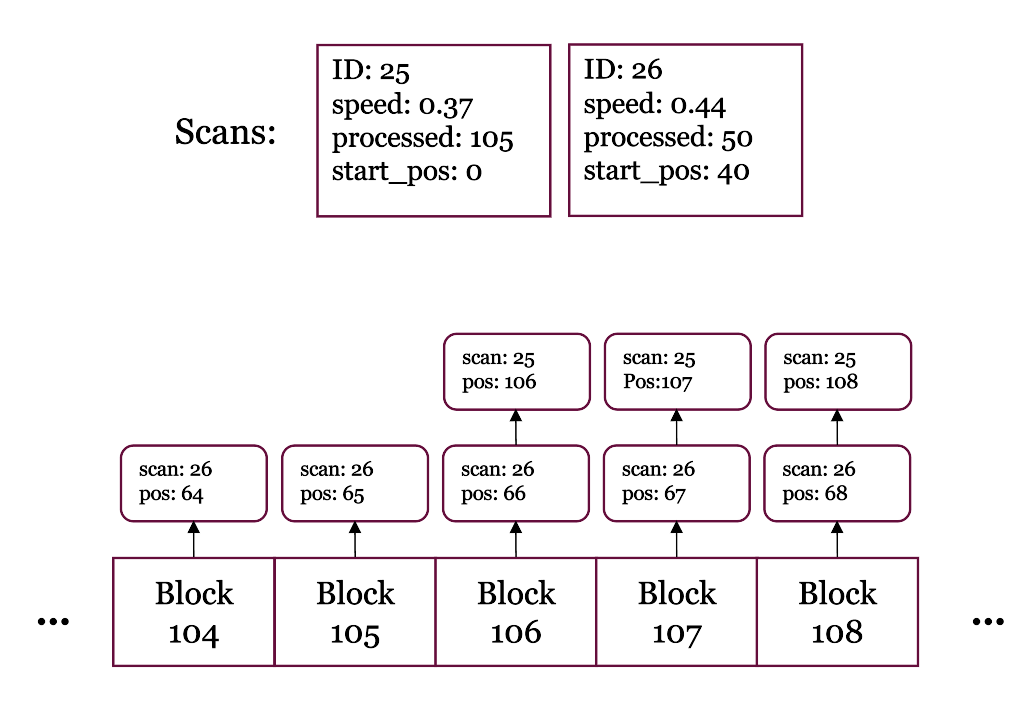
\includegraphics[width=1\columnwidth]{figures/Diagrams/seq_scan_registered_progress.png}
    \caption[PBM sequential scan tracking]{\textcolor{blue}{How PBM tracks sequential scans. A list of relevant scans is tracked for each block in the database. When a scan starts, it adds itself to the list for each relevant block, and removes itself after the scan has passed that block. Time of access for each scan is estimated based on the scan speed and the distance from the scan to the block, based on block position and current scan position. Then the estimated next-access-time of the block is the minimum access time over the list of scans.}}
    \label{fig:scan_tracking}
\end{figure}

\begin{figure}
    \centering
    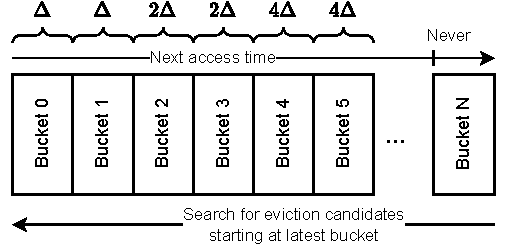
\includegraphics[width=1\columnwidth]{figures/Diagrams/diagrams-approx-PQ.pdf}
    \caption[PBM-PQ's approximate priority queue]{Structure of the approximate priority queue used by PBM-PQ. The time range associated with each bucket increases exponentially for later buckets, and $\Delta$ is the time range of the first buckets.}
    \label{fig:approx-pq}
\end{figure}


\chapter{Sampling-based Predictive Buffer Management}
\label{sec:PBM-sampling}

This chapter presents an alternative buffer management strategy based on sampling that uses the same estimates about future access times as PBM-PQ but removes the need for the approximate priority queue entirely. This improves prediction accuracy for choosing eviction candidates, significantly simplifies the design and implementation, and is more flexible and extensible.

\SetKw{KwReturn}{return}
\begin{algorithm}
\SetAlgoLined
\DontPrintSemicolon
\SetKwFunction{FEvictBlock}{ChooseEvictedBlock}
\SetKwFunction{FEstNextAccess}{EstimateNextAccess}
\SetKwFunction{FScanBlocksUntil}{scan\_blocks\_until}
\SetKwProg{Fn}{Function}{:}{}

\Fn{\FEvictBlock{}}{
    samples $\gets$ array of length $N$\;
    \For{$i \gets 1$ \KwTo $N$} {
       blk $\gets$ random unused block\;
       t $\gets$ \FEstNextAccess{blk}\;
       samples[$i$] $\gets$ (blk, t)\;
    }
    % sort(samples) descending by estimated access times\;
    \For{$i\gets 1$ \KwTo $N$}{
       $s \gets$ sample with highest estimated access time\;
       \eIf{$s$ can be evicted}{
          \KwReturn $s$\;
       }{
          remove $s$ from list of samples\;
       }
    }
    \KwReturn random unused block\;
}\;

\Fn{\FEstNextAccess{blk}}{
  \eIf{blk has registered scans}{
     \KwReturn      
     $\min_{s \in \text{blk.scans}}{\frac{s.\text{\FScanBlocksUntil{blk}}}{s.\text{est\_speed}}}$
     \;
  }{
     \KwReturn $\infty$\;
  }
}\;
\caption{Sampling-based eviction strategy}
\label{alg:sampling}
\end{algorithm}

The sampling-based approach, referred to in this thesis as PBM-sampling, tracks the progress of scans in the same way as PBM-PQ: scans are registered and a list of relevant scans is kept for each block. The change from PQ-based to sampling-based \gls{pbm} is in how it uses the estimated access times to select what to evict. Rather than use a data structure to rank candidates, the sampling-based strategy selects a random group of candidates and use the estimated access times to choose the victim from the selected sample.

Pseudocode for choosing which block to evict is shown in Algorithm~\ref{alg:sampling}. First, the system chooses $N$ random blocks from the cache that are not currently in use, where $N$ is a configurable constant.\footnote{$N=10$ for most experiments in the evaluation.} A block cannot be evicted if it is currently in use, so such blocks must be skipped and something else is selected. The sampling-based approach estimates the next access time for each of the $N$ blocks in the same way as PBM-PQ, by estimating when each active scan will reach the block and considering the scan that is predicted to reach it first. Then from the $N$ sampled blocks, the one with highest estimated next-access-time is returned.

Note that it is possible for the selected block to not be evictable anymore if a concurrent query either already evicted it or started using it. The implementation avoids locking the blocks when they are initially selected to minimize the possible impact on concurrent queries while calculating the access time estimates. To handle this race condition, there is a check at the end for whether the chosen block is still a valid candidate and another block is selected if it is not valid anymore.

This approach is similar in spirit to the learned relaxed Belady approach of \citet{relaxedBelady}. The next part of this chapter justifies why this approach is expected to work well.


\section{Generalizing the Optimal Eviction Strategy}
\label{sec:generalized-MIN}

The most straight-forward approach to mimic Belady's optimal caching policy MIN~\cite{beladyMIN} would be to try to identify the single cache item that will be accessed furthest in the future. However MIN only provides a single choice for eviction when there may be many optimal choices, making this approach more difficult to accomplish than it needs to be. To make the problem easier without sacrificing optimality, consider what MIN will eventually do with the items currently in the cache: any cache item that MIN would evict before that item is next accessed is also an optimal choice for eviction. This is established using the following lemmas:

% could move this to preamble...
\newtheorem{claim}{Lemma}

\begin{claim}\label{lemma:swap-opt}
% This can be generalized more: the policy does not have to be optimal, just that swapping two evictions in this situation will not change the hit rate. But here I only care about the optimal case.
Suppose that $A$ and $B$ are items in the cache at time-step $t_0$, both $A$ and $B$ are next accessed after $t_1$, and some optimal policy (not necessarily MIN) would evict $A$ at $t_0$ and evict $B$ at $t_1$. If the evictions of $A$ and $B$ are swapped -- so $B$ is evicted at $t_0$ and $A$ is evicted at $t_1$ instead -- then the resulting strategy is still optimal.
\end{claim}

\begin{proof}
Since neither $A$ nor $B$ are accessed between $t_0$ and $t_1$ and the rest of the cache contents are unaffected in this time range, swapping the evictions will not change the number of cache hits/misses between $t_0$ and $t_1$. After $t_1$ both $A$ and $B$ have been evicted and the cache contents are now identical to if the evictions were not swapped, so the behaviour after this point is identical to the original policy and there are also no additional cache misses after $t_1$. Thus $B$ would also be an optimal eviction candidate at $t_0$, since swapping these evictions does not occur any extra cache misses.
\end{proof}

Considering the above argument for MIN specifically instead of any optimal policy in general, then $A$ necessarily has a larger next access time at $t_0$ than $B$, since otherwise MIN would evict $B$ before $A$. This argument applies for \textit{all} items in the cache at $t_0$ that MIN would evict before their next access, so using Lemma \ref{lemma:swap-opt} they are \textit{all} optimal eviction choices at $t_0$. I refer to this set of cache items that MIN would evict before their next access as \textit{MIN-optimal}.


\begin{figure}
    \centering
    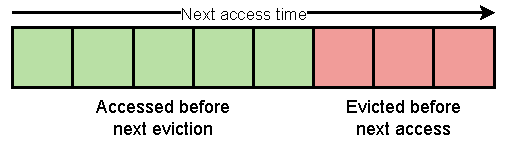
\includegraphics{figures/Diagrams/diagrams-belady-boundary.pdf}
    \caption[Higher next-access-time for MIN-optimal cache items]{Cache items evicted by MIN before next-access have later next-access time than items that will be read from the cache before eviction.}
    \label{fig:belady-boundary}
\end{figure}


\begin{claim}
\label{lemma:opt-greater-next-access}
% Using MIN, all cache items that would be evicted before their next access have later next-access-time than all other items in the cache.
All MIN-optimal cache items have later next-access-time than all items in the cache that are not MIN-optimal. (depicted in Figure \ref{fig:belady-boundary})
\end{claim}

\begin{proof}

Suppose $A$ and $B$ are items in the cache, and $B$ has earlier next-access-time than $A$. If $B$ is MIN-optimal, then $A$ must be as well.

Let $t^\text{evict}_A$ and $t^\text{evict}_B$ be the times when MIN would evict $A$ and $B$ respectively, and let $t^\text{access}_A$ and $t^\text{access}_B$ be the next access times of $A$ and $B$.

Suppose that $B$ is MIN-optimal so $t^\text{evict}_B < t^\text{access}_B$. As previously stated, $B$ is next accessed before $A$ so $t^\text{access}_B < t^\text{access}_A$, and as a result MIN will evict $A$ first so $t^\text{evict}_A < t^\text{evict}_B$. Then by transitivity, $t^\text{evict}_A < t^\text{access}_A$ so $A$ is also MIN-optimal.

Thus it is impossible for a MIN-optimal cache item to have earlier next-access-time than a non-MIN-optimal cache item.
\end{proof}

% [revise next para as it reads oddly: Then...  Then... ??]

Then at any time there are potentially many cache items that are optimal to evict, and some subset of optimal choices have next access times larger than all the other cache items. Based on this, there must be some cut-off time dividing these optimal-to-evict cache items from the rest -- depicted in Figure \ref{fig:belady-boundary} -- which if it were known would be very helpful in identifying good eviction candidates. This is similar to the ``Belady boundary'' described by \citet{relaxedBelady} as the minimum time-to-next-access of all items evicted by MIN. Unfortunately this cut-off time is not known in advance, but it is very useful to know that cache items with later next-access-time have a higher likelihood of being optimal eviction choices. 

Note also that even amongst items that MIN would not evict before their next access, it is still better to evict the one with larger access time. This is proven as part of the proof that MIN is optimal.~\cite{MINOptimality} % in Lemma 1 of the appendix

Thus, evicting the item with highest next-access-time from a sample makes sense and has a reasonably high chance of making an optimal decision assuming next-access-time estimates are accurate, and with a large enough sample. Suppose that the fraction of cache items that are optimal eviction candidates is $p$. Then the probability of making an optimal eviction choice is $1-(1-p)^N$ where $N$ is the sample size. Figure \ref{plot:P-opt-eviction} show the probability of optimal evictions as a function of $p$ for different sample sizes.

\begin{figure}
    \centering
    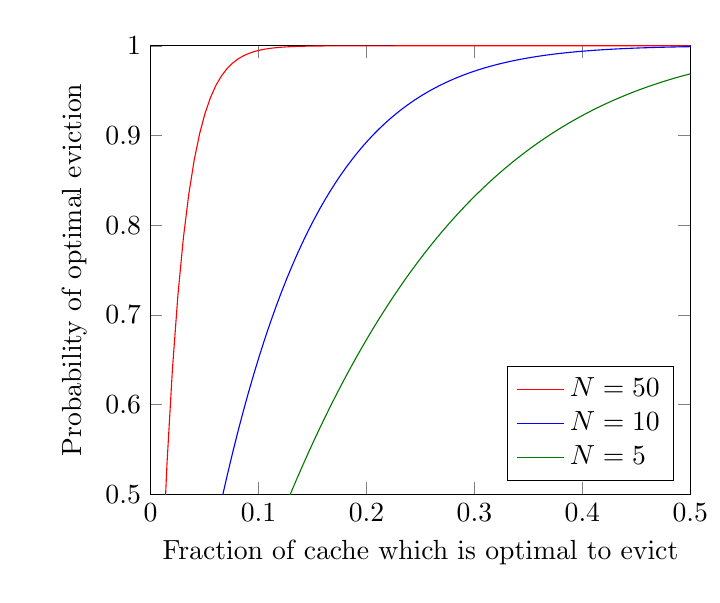
\begin{tikzpicture}
    \definecolor{darkgreen}{RGB}{0,120,0}
    \begin{axis}[
        domain=0:0.5, xmin=0, xmax=0.5,
        range=0.5:1, ymin=0.5, ymax=1,
        samples=100,
        legend pos=south east,
        legend cell align={left},
        xlabel=Fraction of cache which is optimal to evict,
        ylabel=Probability of optimal eviction,
    ]
    \addplot[color=red]{1-(1-x)^50};
    \addlegendentry{$N=50$};
    \addplot[color=blue]{1-(1-x)^10};
    \addlegendentry{$N=10$};
    \addplot[color=darkgreen]{1-(1-x)^5};
    \addlegendentry{$N=5$};
    \end{axis}
    \end{tikzpicture}
    \caption[PBM-sampling probability of optimal decision]{Probability of an optimal eviction decision with $N$ samples}
    \label{plot:P-opt-eviction}
\end{figure}



\subsection{Incompleteness of the generalized policy\label{subsec:gen-belady-incomplete}}

While the strategy of comparing next-access-time to when MIN would evict a cache item described in Chapter~\ref{sec:generalized-MIN} would identify more than one optimal eviction candidate, it is \textit{incomplete} in the sense that it does not identify \textit{all} possible optimal candidates, even with perfect knowledge of future accesses.

As an example of this: consider a cache of size 2 that initially contains items $A$ and $B$, and a sequence of accesses for item $C$, $A$, $B$, $A$. MIN would evict $B$ to read $C$, read $A$ from the cache, then evict $C$ to read $B$, and finally read $A$ from the cache again. This results in 2 evictions over the whole sequence. In the first step when $C$ is read, $A$ will be accessed before MIN would choose to evict it so only $B$ is MIN-optimal, not $A$.

However, it is possible to evict $A$ in the first step and still end up with an optimal sequence of evictions. Again starting with $A$ and $B$ in the cache, evict $A$ to read $C$, then evict $C$ to read $A$, and for the last two reads $B$ and $A$ are cached. This sequence of accesses also has only 2 evictions, so it is optimal, but it does not evict only MIN-optimal candidates. Thus the generalized policy is \textit{incomplete} in that it does not identify all possible optimal eviction decisions.

\subsection{Eviction times of the generalized policy}
An interesting observation is that the generalized policy will have its cache misses and evictions at the same time steps in the access sequence as MIN. However, for the example in Chapter~\ref{subsec:gen-belady-incomplete} of an optimal sequence of evictions that does not follow the generalized optimal policy, the evictions occur earlier in the sequence, at the first and second access instead of first and third. 

% This raises a few follow up questions that I do not explore in this thesis:
% \begin{enumerate}
%     \item Does MIN always have the latest possible evictions?
%     \item Is there sequence of evictions that does not follow the generalized optimal policy, but is still optimal and does not evict earlier than MIN?
%     \item Knowing the future accesses, is it possible to efficiently identify \textit{all} optimal eviction choices at a particular time?
% \end{enumerate}


\section{Sampling-based PBM: Benefits and Trade-offs\label{sec:sampling-advantages}}

To maximize performance, the buffer management policy should maximize the hit rate of block accesses while minimizing CPU overhead. This includes minimizing the time to choose what to evict, time to maintain metadata, and limit time holding locks so that threads can allocate cache blocks concurrently without waiting for each other.

PBM-PQ~\cite{pbm} trades off prediction accuracy by using the approximate priority queue to avoid the high CPU overhead of maintaining an exact priority queue, and allowing estimates to become stale. Sampling-based \gls{pbm} benefits from removing the central priority-queue data structure, allowing it to achieve better hit rate without additional CPU overhead.


\textbf{Simplicity}: The most obvious advantage after implementing both policies is increased simplicity -- sampling removes the entire approximate priority queue data structure along with the maintenance required to shift the buckets periodically and ensure block groups are in the correct bucket as blocks move in and out of the cache or their registered scan set changes.

With sampling, all of this is removed and the eviction logic changes, with almost nothing added. In the PostgreSQL implementations, PBM-sampling has about 600 fewer lines of code than PBM-PQ.


\textbf{Freshness of access-time estimates}: The sampling-based approach computes next-access-time estimates as late as possible -- only when a block is being considered for immediate eviction -- so the estimates it uses are based on the most up-to-date information available.

In contrast, the PQ-based approach calculates estimates only when the set of scans registered for a block changes potentially causing the block to be moved to a different bucket of the approximate priority queue. If the initial estimated access times were perfectly accurate this would not matter, but in practice the scans will change speed over time depending on various run-time factors. A block could remain in the cache for minutes at a time without its position in the queue being recalculated, leaving plenty of time for estimates to drift. Less accurate estimates lead to worse eviction decisions and, by extension, worse performance.

\textbf{Accuracy of access-time estimates}: The approximate priority queue considers blocks in the same bucket as equivalent when deciding what to evict, with buckets further in the future -- which are checked first for potential eviction candidates -- representing exponentially larger time ranges. Sampling compares the exact estimated next-access, however, it considers only a small sample of blocks for each eviction compared to PBM-PQ, which chooses among all blocks in the cache. Both methods sacrifices some precision that prevents them from always picking the best block to evict, even if the estimates were completely accurate. Chapter~\ref{sec:generalized-MIN} discusses how to reason about the precision of the sampling-based strategy.  % less clear how to reason about it for PQ-based

\textbf{Extensibility}: PBM-PQ is designed for workloads with mostly sequential scans, and the approximate priority queue makes it difficult to extend it to other workloads. \citet{pbm} suggest, but do not implement, a way to incorporate frequency statistics to handle blocks that are not requested by sequential scans but may be accessed by other methods for hybrid workloads. Their proposal requires an entire new data structure that is processed differently from the existing priority queue because the existing structure assumes the priorities (time to next access) change in a specific way over time. 

With sampling, a complex data structure is not required for ordering blocks, so it is much easier to extend to support other workload types. Unlike with PBM-PQ, no extra work is required to make use of improved assess time estimates using new sources of information.

\textbf{Tunability}: With sampling, the sample size can be changed at run-time without interrupting the workload in any way. Caching policies must compromise between CPU cost and hit rate, and adjusting the sample size is an easy way to do this with intuitive impact: more samples should increase the hit rate, but increases the per-eviction CPU cost.

With PBM-PQ, the number of buckets in the queue and the time ranges represented by each bucket are adjustable. However, changing these parameters requires modifying the data structure including potentially recalculating access time estimates, and it is not as obvious when more buckets or a different time range would be beneficial. These adjustments improve the precision, but do not help when estimates become stale.


\textbf{Concurrency:} PBM-sampling does not have a central data structure used for making eviction decisions, so evictions can be done in parallel from multiple processes with low frequency of one thread having to wait for another (one thread will have to wait if two threads randomly sample the same buffer at the same time). Using the approximate priority queue prevents concurrent evictions, which could potentially limit the scalability at high levels of concurrency. PBM-PQ works around this limitation by evicting many blocks at once so that allocating a buffer usually does not need to wait.% and in the experiments the centralized data structure of the PQ-based implementation does not seem to actually impact performance.

 % ... cpu overhead more generally? ... Measured average CPU overhead of choosing eviction candidate lower for sampling, but not as low as clock. -- calculates priorities more frequently ...


% \textbf{Disadvantages}: ... are there any? (other than weird issues where it does not help on HDD...)



\chapter{Extending and Enhancing Sampling-based PBM}
\label{ch:extending-sampling}
This chapter describes improvements to PBM-sampling, some of which are general improvements for all workloads and others allow PBM-sampling to perform well on workload types beyond what PBM-PQ specialises in.

\section{Bulk Eviction\label{sec:sampling-bulk-eviction}}

PBM-PQ evicts several pages at once to amortize the CPU cost of eviction.~\cite{pbm} With sampling, there is not a direct CPU benefit to evicting multiple blocks at once, but better hit rate is achievable for the same CPU cost with a similar bulk eviction technique.

Rather than choosing $N$ buffers from the cache and evicting only one each time a buffer is allocated, consider taking a sample of $kN$ buffers and evicting the $k$ buffers from the sample with largest next-access time. This technique considers the same $kN$ buffers over a sequence of $k$ buffer allocations, but can make better eviction decisions by considering them all together rather than separately.

With separate single evictions, it is possible that one sample may not contain any good candidates resulting in a bad eviction, while another sample may contain multiple good eviction candidates but will select only one. With bulk eviction, it is as if one can take a surplus good eviction candidate from a different recent or near-future sample instead of evicting the bad candidate, thus reducing the over-all rate of bad eviction choices. Using the example in Figure \ref{fig:multi-eviction}, the first eviction samples two good eviction candidates while the second eviction samples only items that should be kept in the cache, so with single eviction it would end up making a bad eviction. Using bulk eviction for this scenario, the same sampled cache items from multiple consecutive evictions are considered together allowing both good candidates from the first single-eviction sample to be evicted and avoiding evicting something which would optimally be kept in the cache. Appendix~\ref{sec:sampling-probabilities} analyses and demonstrates this benefit mathematically.


\begin{figure}
    \centering
    \begin{subfigure}{\columnwidth}
        \centering
        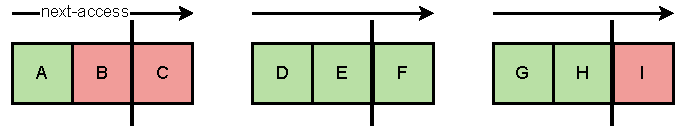
\includegraphics[width=\columnwidth]{figures/Diagrams/diagrams-multi-eviction-a.pdf}
        \caption{Multiple single evictions each evict the single item with latest next-access from a limited sample.}
    \end{subfigure}
    \vspace{5pt}
    \begin{subfigure}{\columnwidth}
        \centering
        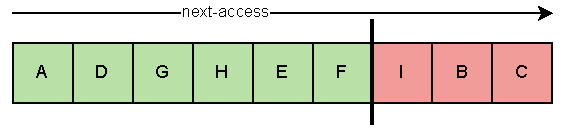
\includegraphics[width=0.8181818\columnwidth]{figures/Diagrams/diagrams-multi-eviction-b.pdf}
        \caption{Bulk-eviction considers the same samples, with a better set of eviction choices.}
    \end{subfigure}
    
    \caption{Bulk eviction example with $N=k=3$. The colour identifies MIN-optimal eviction candidates as in Figure~\ref{fig:belady-boundary}, and items to the right of the vertical bars are chosen for replacement.}
    \label{fig:multi-eviction}
\end{figure}

With this technique the total number of samples chosen -- and therefore next-access estimates computed -- stays the same compared to single-eviction, so the CPU cost is practically the same, but the eviction decisions are better so hit rate is improved.


% With more evictions together there is a larger gap between when eviction decisions are made and when the block is actually replaced in the cache. With too many evictions at once this gap means evictions decisions are effectively made earlier than the actual eviction, running the risk of bad eviction decisions based on old data, but for a small number of evictions at once the time to replace all blocks chosen for eviction is very small.



\section{\label{sec:frequency-stats}Frequency Statistics}

\citet{pbm} mention, but do not implement, an extension to PBM-PQ using frequency statistics to prioritize cache blocks that are not requested by any active sequential scans. This is not expected to help for workloads with only long-running sequential scans, but could be useful for smaller tables and index lookups. The method proposed by \citet{pbm} is to store a few recent access times for each block, and store non-requested blocks in a separate set of buckets corresponding to the inter-access time. The second set of buckets ages over time, equivalently increasing the estimated time-to-next-access of these blocks.

This thesis pursues this proposal by developing a similar idea to track frequency statistics in PBM-sampling that is much easier to implement as discussed in Chapter~\ref{sec:sampling-advantages}. In PBM-sampling, the system tracks an exponentially weighted moving average of the time between accesses (inter-access time) for each block in the cache. With sampling no special data structures are needed to handle this scenario, just some extra fields in the existing buffer headers. If the time-since-last-access is less than the average inter-access time, the frequency-based time-to-next-access is estimated to be the average inter-access time. Once the time-since-last-access exceeds the average inter-access time, the time-since-last-access is used as the estimated time-to-next-access instead to decrease the relative priority of these blocks over time. 

If a block is also registered by a sequential scan, the resulting next-access estimate is the minimum of the frequency-based and registered-scan-based estimates.

These stats are only kept for blocks currently in the cache, so newly loaded blocks will not have an inter-access time since they have been accessed only once. Newly loaded blocks are therefore more likely to be evicted prematurely if they are not also requested by a sequential scan. This is mitigated with sampling since, on average, some time will pass before the blocks will be sampled. The next sub-chapter discusses another method for handling the case of non-requested blocks.

\section{\label{sec:lru_nr}Fallback to LRU}


The original implementation of PBM-PQ \cite{pbm} uses \gls{lru} to prioritize amongst blocks that are not requested sequentially.\footnote{The PostgreSQL implementation of PBM-PQ in this thesis takes a different approach, discussed in Chapter~\ref{sec:pbm-pq_postgres}.} With the sampling-based strategy, the frequency statistics described in Chapter~\ref{sec:frequency-stats} mostly serves the same purpose, but as mentioned it has a blind-spot for blocks that are new to the cache and have not yet been accessed multiple times. A technique that can be used to improve this case is to use \gls{lru} as a tie-breaker for blocks that are not requested sequentially and do not have frequency statistics. If multiple sampled blocks are not requested sequentially and do not have frequency statistics, the system will prefer to keep the ones that have been accessed more recently and evict the one accessed least-recently. % or, if freqency stats are disabled it can use this instead


\section{\label{sec:index_scans}Index scans}

So far the discussion has been mainly about sequential access patterns. Sequential scans are the most efficient way to read a large data-set when most of the data is needed to answer a query, but secondary indexes can greatly reduce I/O and CPU cost for workloads where this is not the case. PostgreSQL supports various types of indexes, so they should also be considered to inform caching decisions.

Unfortunately, index scans do not generally have a predictable order for accessing secondary storage, so they are not as easy to predict as sequential scans. There are, however, a few situations where the information from an index scan may be useful to help make eviction decisions.

\subsection{\label{sec:bitmap_scans}Bitmap index scans}

In PostgreSQL, any index can be scanned as a bitmap scan. In this case, the system first reads only the index and constructs a bitmap indicating which tuples might match the query predicate. The table is then scanned in sequential order, using the bitmap to skip blocks that do not contain any matching tuples. Bitmap scans can be selected by the query planner for any type of index, but certain index types can only be used with bitmap scans. Most notably, PostgreSQL's block range indexes (BRIN) always use bitmap scans. BRIN splits the table into ranges of blocks and stores a summary of each range, which can be compared to the query predicate to quickly rule out all tuples from a range. The default form of BRIN is a min-max index, where the summaries store the column's minimum and maximum value for each range of blocks, and it also supports bloom filter summaries and a few other strategies for specific data types.

Bitmap scans are the best-case for index scans with predictive buffer management: the order is predictable and the set of blocks to be retrieved is known early, after constructing the bitmap. It is easy to support bitmap scans in both sampling-based and priority-queue based \gls{pbm} as the only necessary change is to how the scan is initially registered. The \gls{pbm} registration happens after the scan operator constructs the bitmap, and the bitmap itself is used to determine which blocks will be scanned and when, but the rest of the implementation is the same as for sequential scans.

The original implementation of PBM-PQ supports automatically created min-max indexes in a similar way~\cite{pbm}, but PostgreSQL's bitmap scans are more general and apply to more types of indexes.


\subsection{Trailing index scans}
\label{sec:idx_trailing}

Certain index types -- such as B-tree indexes -- return their results in sorted order. Thus two independent index range scans with overlapping ranges will visit the tuples from the shared part of the range in the same order. When there are concurrent index range scans on the same relation, the system can detect the shared scan range and use information from one scan to know what the next scan will access.

The way a trailing index scan is detected involves marking blocks as they are accessed by the leading scan for the trailing scan to detect when it reaches the same point. When an index scan accesses a block it records in the buffer header: the current time, which tuple from the block was accessed, and which index is used. When another index scan reaches the same tuple, it checks the mark to determine whether it is following another scan. If the mark is for the same index and the same tuple, the scan knows it is trailing the scan that left the mark and can calculate how far behind it is based on the recorded timestamp. It then notifies the leading scan that it is trailing with a certain delay, and the leading scan will also start marking blocks it accesses with the time it estimates the trailing scan will also reach that block. Estimating next-access-times will now use the estimate left by the leading scan if this estimate is less than the access time suggested by other factors.

% ... Alternate (unimplemented) idea for detecting trailing scan: Modify the B-Tree structure to know the current position w.r.t. the index order. Can do this by modifying the internal nodes to store the size (\# of leaves) in each subtree. When searching the tree for the starting point of the range, add up the number of leaves in the subtrees left of the search path to know the position of the first tuple in the index order. Then multiple scans can be ordered by their position to determine how many tuples apart they are in the index order.


\subsection{Almost-sequential index scans}
\label{sec:idx_seq}

Some columns in a table are highly correlated with the physical order of the table. Such columns are good candidate for BRIN indexes, but a B-Tree index can make sense when the query optimizer also wants to sort by that column efficiently. Due to the correlation between the column order and physical order, even an index scan on the column will access the disk blocks in a mostly-sequential order. The PostgreSQL optimizer already has statistics for how correlated an index scan will be with the physical order, so when the correlation is high the index scan can be treated more like a sequential scan. Then the system can estimate when a specific scan will reach a specific block based on the scan's current position and distance between the current and target block, and how fast the scan is progressing.

% Why this might not work well:
%  - for the microbenchmark I came up with, the scan jumps backwards 4k blocks from one key to the next (I only looked at a tiny part of the data, maybe worse over-all). 
%  - so at any time, there is ~320 MiB that could be accessed in the very-near future, which is too much to reasonably keep cached per query.


% \textbf{Inverse frequency}: ...

\subsection{Random access}

For less predictable accesses, such as point look-ups or index scans with no correlation between index and physical order, it is much more difficult to reliably estimate next-access-times. In these scenarios, the frequency statistics from Chapter~\ref{sec:frequency-stats} are a reasonable heuristic for detecting hot-spots in the data.



\chapter{\label{sec:pbm-pq_postgres}Implementation in P\MakeLowercase{ostgre}SQL}


This chapter describes the implementation of predictive buffer management in PostgreSQL. This includes implementing both the sampling-based approach and the PQ-based approach that is not implemented in an open source system, into PostgreSQL. Having both implementations in PostgreSQL allows us to conduct an apples-to-apples evaluation and  comparison of the two approaches. The differences between the implementation in \cite{pbm} and this thesis will be pointed out in the relevant parts of this chapter.

%Note that due to differences between PostgreSQL and Actian Vector, there will be certain differences between the PostgreSQL implementation of PBM-PQ and what would have been implemented by \cite{pbm}. These differences will be pointed out in the relevant parts of this chapter.


\section{PostgreSQL's Existing Buffer Replacement}

As previously mentioned, PostgreSQL uses a clock-sweep strategy for cache replacement. PostgreSQL has an in-memory array of buffer headers -- separate from the buffer contents -- that include a usage count used by clock-sweep as well as other fields, including a reference count, identifier of which block is in the buffer, and whether it needs to be written back to secondary storage among others.

When a buffer is allocated, the system first checks a linked list of free buffers, and if that is empty it runs the clock-sweep algorithm. The clock-sweep strategy involves reading and atomically incrementing a global index into the array of buffer headers (the ``clock hand''), and checking the buffer at that index. If the buffer has a zero usage count and is not in use, it is selected for replacement with the new buffer. Otherwise, its usage count is decremented and the process is repeated until a suitable buffer is chosen for replacement.

PostgreSQL's cache replacement selection is very simple, with only a few global variables, a global linked list of free buffers, and an extra field in each buffer header. To support a predictive buffer management strategy, some changes are required to track the extra metadata.


\section{Changes to PostgreSQL to Support PBM}

First, some additional data structures are required. This includes a set of the active scans and a hash map to track the set of registered scans for each block in the database, as well as some global metadata and other data structures for managing the shared memory used by the \gls{pbm} data structures. The hash map of blocks additionally has its entries linked together in order by block number so that initially registering a scan requires only a single hash lookup to register with all blocks. The PostgreSQL implementation of PBM-PQ additionally adds the approximate priority queue as a global data structure. The existing buffer headers have some additional fields added to track frequency statistics for cached blocks, and pointers to the relevant entries in the other shared data structures to facilitate low-latency computation of next-access estimates. 

Scan operators are also augmented with extra fields to track their progress -- both current position and speed -- and a pointer to the corresponding structure in shared \gls{pbm} metadata used by access-time estimates. When a sequential scan first starts it uses the hash map of blocks to find the blocks it must register with. At run-time, scans update their local statistics as they go and periodically update the shared statistics to keep them up-to-date, as well as un-registering the scan from blocks that have been processed and will not be needed again by that scan.


\subsection{Details of PBM implementation}

This sub-chapter provides more details on specific aspects of the PostgreSQL implementation.


\textbf{Block groups:} Both \gls{pbm} approaches store metadata about active scans for every block in the database. With PostgreSQL's default 8~KiB block size, even a few tens of bytes per requested block per scan will require this metadata to consume significant amounts of memory for a large database when many scans are active. To reduce the memory footprint, consecutive blocks of each relation are grouped into \textit{block groups} of a constant size and \gls{pbm} metadata for sequential scans is stored at the block group level instead of for every individual block. The PBM-sampling implementation uses a default block group size of 1~MiB, so 128 consecutive blocks share metadata about requesting scans. 1~MiB is chosen partially to correspond with the granularity of PostgreSQL BRIN indexes, which by default also store statistics about 1~MiB chunks of data. The original PBM-PQ implementation~\cite{pbm} would not need such block groups as they already uses a much larger default block size. \cite{vectorDocs}  % ... block groups get stored in the PQ buckets, not the buffers directly

The block group statistics are stored in a hash map and block groups for the same table form a linked list such that they can be traversed sequentially without multiple hash table look-ups when registering a sequential scan. % this is simplified: the block groups are actually allocated in fixed-size chunks and those chunks are linked together. This saves a bit of memory and reduces pointer chasing when scanning through the block groups, though it is probably insignificant.
When a block is loaded into the cache, the hash map is used to find the associated block group. A pointer to the block group is stored in the buffer header to avoid hash look-ups later when estimating the next access time of the cached block. For the PQ-based implementation the block group must also store a list of currently cached blocks from the group, so that the actual blocks can be evicted from the cache when the block group is chosen for eviction. 

% (for sampling: block->group pointer is used to estimate access time of a block. For pq-based: it is used to remove the buffer from the group later when buffer is evicted)


\textbf{Bulk eviction:} \citet{pbm} state that their implementation of PBM-PQ evicts ``groups of 16 or more'' buffers at once to amortize eviction cost. In the PostgreSQL implementation of PBM-PQ, all buffers from the relevant bucket are selected for eviction, which are then placed on PostgreSQL's existing free-list to be replaced as needed. This decision was made primarily to reduce complexity of the eviction method. On sequential workloads where items will be fairly evenly distributed among the different buckets this should not have much impact, but it will change the behaviour on non-sequential workloads where the approximate priority queue classifies everything as not requested: the description from \cite{pbm} would behave like \gls{lru} in this case while the PostgreSQL implementation will be more similar to \gls{fifo}.

The sampling-based approach does not need to amortize eviction cost, which is already very low with a small sample size. There are some benefits to bulk eviction as discussed in Chapter~\ref{sec:sampling-bulk-eviction} but with the default configuration, PBM-sampling evicts only a single buffer at once.

% reason for PBM-PQ evicting a whole bucket at once:
%  - the block-group makes it more complicated to only evict part of the bucket. Some blocks from the bucket could be pinned preventing the group from getting removed from the bucket.
%  - It also is not evicted immediately, only placed onto the free list, so over-evicting is not a big concern since they are still usable until the space is actually needed.


\textbf{Scan ranges and bitmap scans:} As discussed in Chapter~\ref{sec:bitmap_scans}, the PostgreSQL implementation handles min-max indexes by tracking all bitmap scans in a manner very similar to sequential scans. This implicitly supports other bitmap-only indexes and scenarios where a bitmap scan is used for other index types that \cite{pbm} does not handle. The \gls{pbm} implementation treats bitmap scans much like sequential scans, except the bitmap is used to determine which block will be accessed and should or should not be registered.


\textbf{Index scans:} Unlike sequential and bitmap scans, where the scan is registered with each block group, non-bitmap index scans are registered once and store statistics about the scan in a hash map keyed by table ID with a list of active scans for each table. When a block is loaded into cache, a reference to the list of index scans on the relevant table is stored in the buffer header to avoid hash look-ups each time the next-access-time is recalculated.


\textbf{Frequency statistics:} The average inter-access time is tracked in new fields added to the buffer headers. These fields are updated when a block is requested and found to be already present in the buffer cache.


\textbf{Shared memory and concurrency:} A challenge in the PostgreSQL implementation of both forms of \gls{pbm} is dealing with PostgreSQL's shared memory implementation. PostgreSQL uses separate processes for each client connection, and more than one process for the same client if a parallel query plan is used. Using separate processes instead of separate threads in the same process makes sharing the \gls{pbm} data structures between all parallel tasks difficult. Shared data structures in PostgreSQL must be allocated in shared memory when the database is started, limiting the ability to scale the memory used by \gls{pbm} data structures. The implementation deals with this case by over-provisioning shared memory for \gls{pbm} data structures. When bits of shared memory is no longer needed, such as when a scan completes and its \gls{pbm} metadata could be freed, the \gls{pbm} implementation keeps track of the old allocations to be reused by the next scan.
%This is a limitation of the PostgreSQL implementation that should not be an issue in newer systems running in a single process.


% \textbf{other system-level differences:} column store vs not, synchronized sequential scans, ...




\chapter{Evaluation}
\label{ch:evaluation}

This chapter presents the evaluation of the proposed sampling-based predictive buffer management policy, starting with the evaluation methodology followed by presentation and discussion of results. Note that this is the first implementation and comparison of predictive buffer management policies in an open source system, and PostgreSQL in particular.

\section{Methodology}
Experiments are run on a Ubuntu 20.04.3 LTS server with two 6-core Intel E5-2620v2 CPUs with hyperthreading enabled, 32 GiB of RAM, and a 400 GB Intel S3700 SSD with an ext4 file system. A modified version of BenchBase~\cite{BenchBase} is used as a workload generator for the experiments.
% HDD is: 1 TB ST1000NM0033-9ZM hard drive
% SSD is: 400GB Intel S3700 SSD

% using: `hdparm -i /dev/...`, `sudo lshw -class disk`

Most experiments measure cache hit rate, workload completion time, and I/O volume for different caching policies at different levels of parallelism or with different amounts of memory available. I/O volume isolates the benefits of the improved cache management strategy, while hit rate and run-time provide a more complete picture of the performance. The caching policies compared are PostgreSQL's existing clock-sweep strategy, the PostgreSQL implementation of PBM-PQ, and PBM-sampling configured in a variety of settings.

Hit Rate is measured using PostgreSQL's built-in statistics, automatically retrieved from the \verb|pg_statio_user_tables| system view by BenchBase.

Unless stated otherwise, the available system memory is limited using Linux cgroups. This prevents the OS from caching the entire data set and effectively bypassing secondary storage.

% Each experiment is run multiple times with different random seed for the workload generator. Graphs show the average value with 95\% confidence intervals represented by the error bars.
Each data point plotted is the average from at least 5 independent experiment runs. The error bars show 95\% confidence intervals around the averages.


\section{Sequential Microbenchmarks\label{sec:eval-seq-micro}}





The first set of experiments is a microbenchmark intended to measure the performance impact of the buffer management strategy on sequential- and bitmap-scan heavy workloads. These are similar to the microbenchmarks in \cite{pbm}. %, and serve primarily to compare sampling-based PBM to PBM-PQ on the workloads where PBM-PQ is expected to work well. These are also used to evaluate the impact of additional changes made to the sampling-based strategy.


These experiments are based on TPC-H~\cite{tpch} at scale factor 10. At this scale factor, the \verb|lineitem| table takes approximately 8.6 GiB, and the whole dataset is around 10 GiB without indexes. For this experiment, the \verb|lineitem| table has min-max indexes on the \verb|l_shipdate| column, which is used as the filter for queries, and the table is clustered by \verb|greatest(l_receiptdate, l_commitdate)|. This clustering causes the \verb|l_shipdate| column to be correlated, but not completely sorted, with the physical order, so the min-max index can actually be used effectively. This clustering is to simulate a more realistic physical order than the random order generated by BenchBase's TPC-H implementation. In a real data-set the date columns would correspond with when the row is created or last updated that in turn determines the physical order.\footnote{PostgreSQL generally appends new or updated rows at the end of the table, but can reuse space from previously deleted or updated rows, so the physical order will not perfectly correspond with last-updated time.}

The workload runs several parallel query streams, each executing a fix number of queries. To isolate the impact on a workload with only sequential and bitmap scans, the queries used are modified versions of TPC-H Q1 and Q6 as in \cite{pbm}, which are aggregations on \verb|lineitem| with a filter by \verb|l_shipdate|. Each query uses a different randomly selected range of \verb|l_shipdate| including roughly 30\% of rows in the table.

% For these experiments, the queries are modified versions of TPC-H Q1 and Q6, 
% which only read the \verb|lineitem| table with a filter by \verb|l_shipdate| selecting a random range including roughly 30\% of the rows.

% The \verb|pg_prewarm| postgres extension is used to fill the cache with data from the \verb|lineitem| table before the experiment begins rather than start with an empty cache.



\subsection{Comparing Different Levels of Parallelism}
\label{sec:experiment_micro_parallelism}


% SEQUENTIAL PARALLELISM
\begin{figure}[p]
\centering
\begin{subfigure}{0.45\textwidth}
    \centering
    \includegraphics[width=\textwidth]{figures/seq_micro/Hit rate vs parallelism - Sequential Scan Microbenchmarks.tikz}
    \caption{Effect on Hit Rate}
    \label{fig:seq_micro_parallel_hitrate}
\end{subfigure}\hspace{0.05\textwidth}%
\begin{subfigure}{0.45\textwidth}
    \centering
    \includegraphics[width=\textwidth]{figures/seq_micro/IO volume vs parallelism - Sequential Scan Microbenchmarks.tikz}
    \caption{Effect on I/O Volume}
    \label{fig:seq_micro_parallel_iovol}
\end{subfigure}

\vspace{20pt}
\begin{subfigure}{0.45\textwidth}
    \centering
    \includegraphics[width=\textwidth]{figures/seq_micro/Time vs parallelism - Sequential Scan Microbenchmarks.tikz}
    \caption{Effect on Run-time}
    \label{fig:seq_micro_parallel_time}
\end{subfigure}%\hspace{0.05\textwidth}%
% \begin{subfigure}{0.45\textwidth}
%     \centering
%     % \includegraphics[width=\textwidth]{figures/manual_graphs/seq_runtimes.tikz}
%     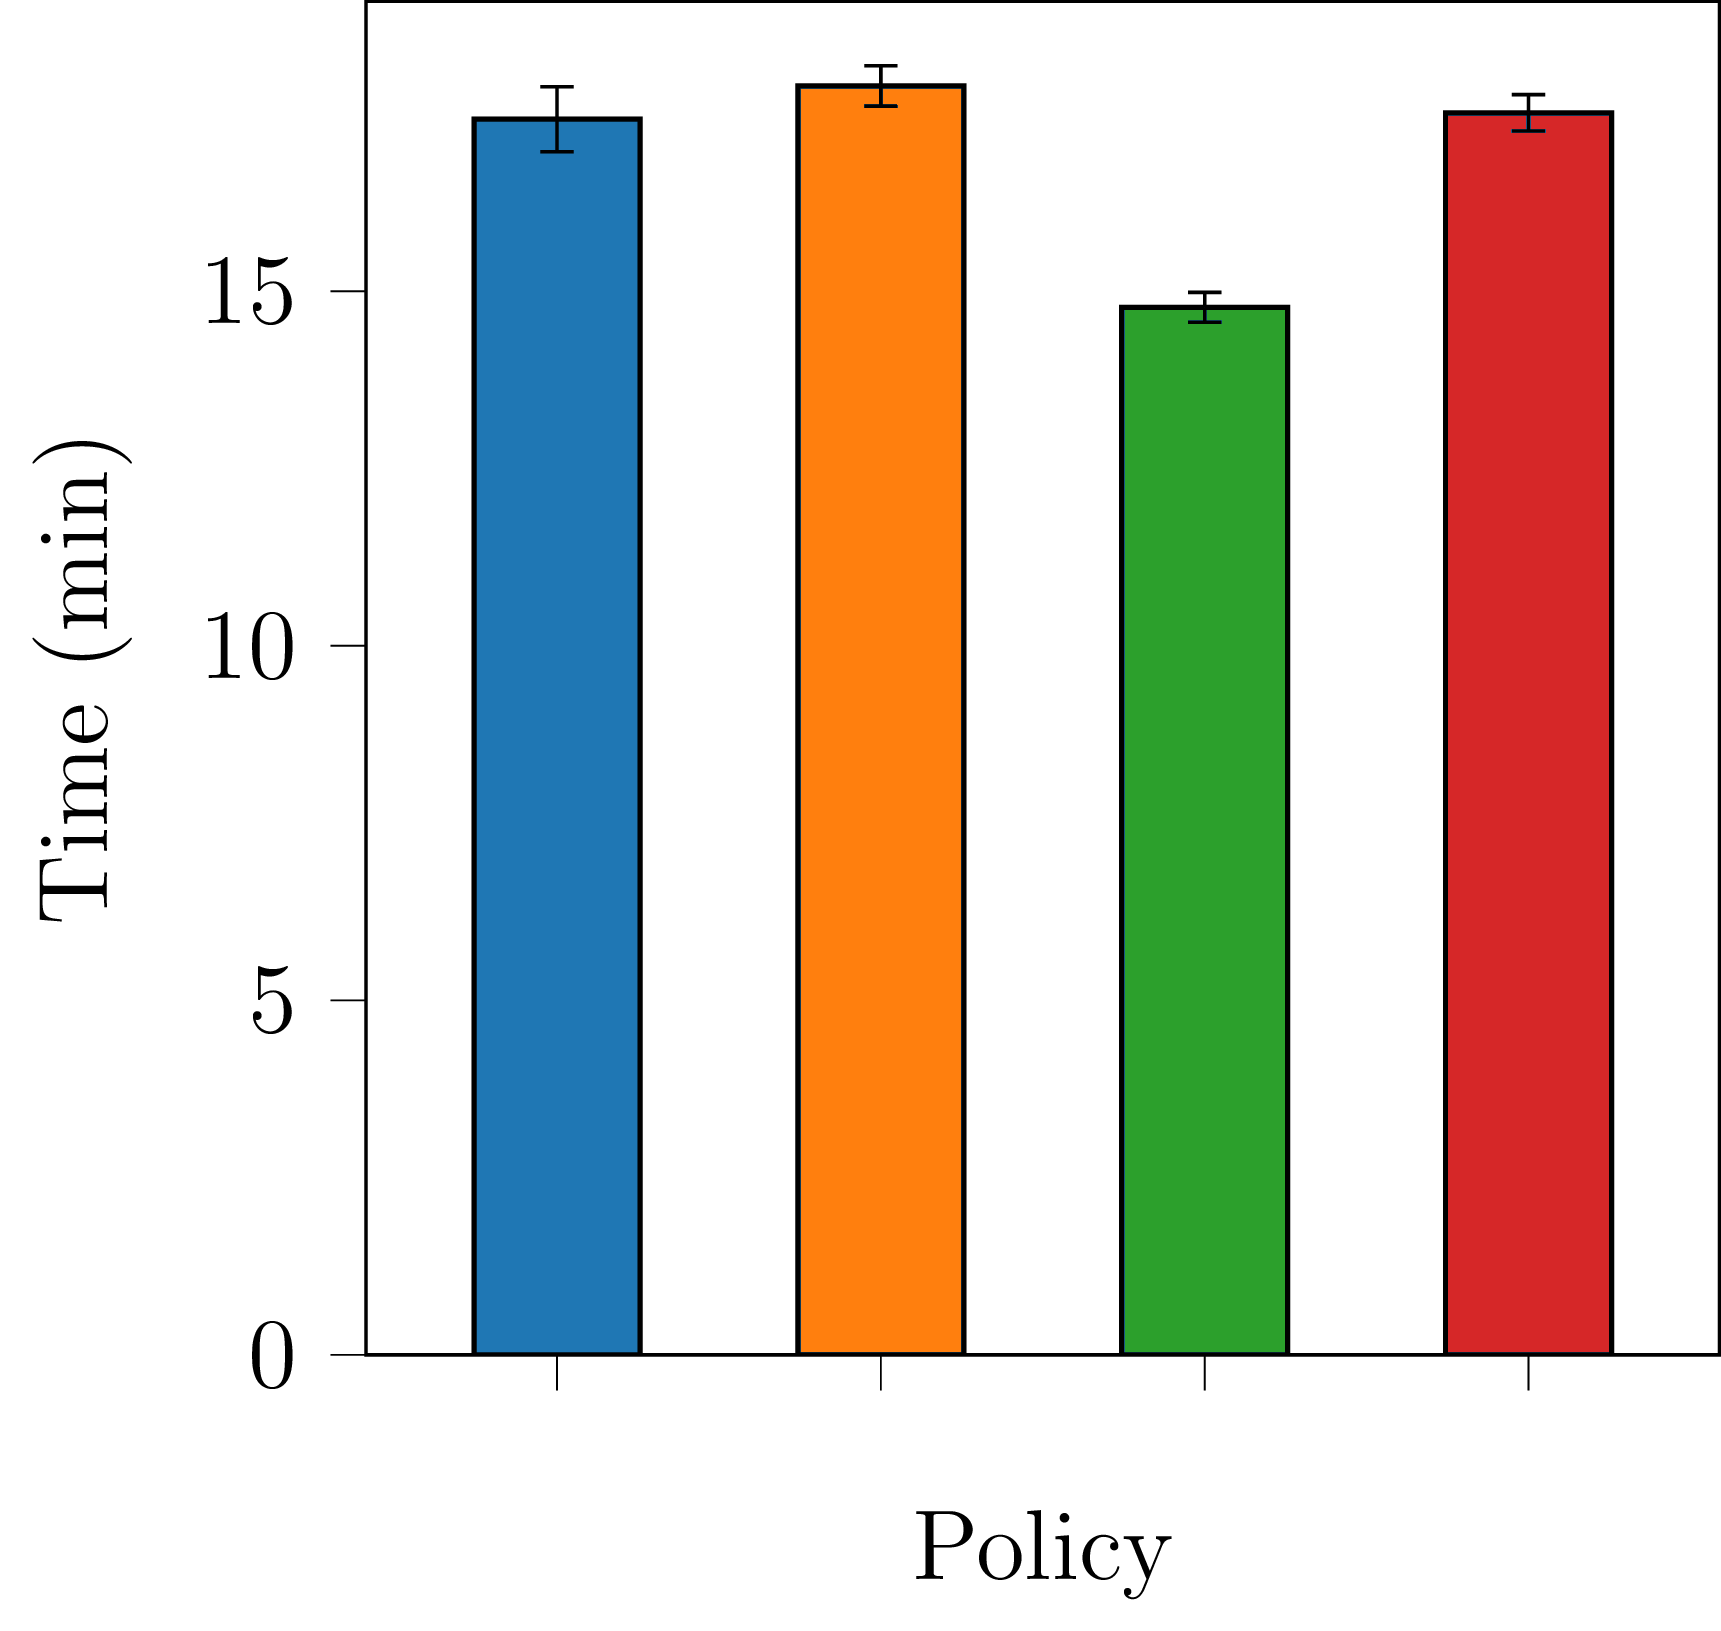
\includegraphics[width=\textwidth]{figures/manual_graphs/seq_runtimes_bar.png}
%     \caption{Run-times at 16 parallelism}
%     \label{fig:seq_micro_runtime_bar}
% \end{subfigure}

\caption{Sequential Microbenchmarks -- Parallelism}
\label{fig:seq_micro_parallelism}
\end{figure}


For this experiment the number of concurrent query streams varies from 1 to 32, with 16 queries per stream each scanning 30\% of the table to measure how the different caching strategies scale with parallelism. PosgtreSQL is configured with 2.5~GiB of cache memory (approximately 30\% of the data size), with available system memory limited to 3~GiB to prevent the OS from caching the whole data set. % some extra memory needed by PostgreSQL for non-cache stuff, hopefully this is obvious enough to not state.

% Revised/additional 2 paras follow.

% Figure~\ref{fig:seq_micro_parallelism} shows the results, with PBM-sampling using 10 samples and no bulk eviction. Since the true test of how well a technique works is how much I/O does its cache management strategy reduce, the focus will be on I/O volume, i.e., I/O savings resulting from using the sampling-based techniques.  To provide a more complete picture, I also show hit rate and workload completion time curves.

% For almost all parallelism levels higher than 2, PBM-sampling delivers significant I/O reductions of about 60 GB over PBM-PQ, which amounts to about 20\% at parallelism level 16 (and 40\% at parallelism level 8 and about 18\% at parallelism level 32).  This I/O reduction is accompanied by higher hit rates and reduced workload completion times. This general trend also holds for the other policies except that PostgreSQL's Clock-Sweep algorithm reduces the gap at parallelism levels higher than 16. 
%  Note that this is the first comparison of all policies against an open source system, and PostgreSQL in particular. 

%  Revised/additional 2 paras ended.
 
Figure~\ref{fig:seq_micro_parallelism} shows the results, with PBM-sampling using 10 samples and no bulk eviction. For all parallelism levels, PBM-sampling without frequency stats delivers significant I/O reductions. At Parallelism level 8 the reduction is about 60 GiB over PBM-PQ, which is nearly 30\% lower, and at parallelism level 32 PBM-sampling saves 11\% I/O volume over PBM-PQ. This I/O reduction is accompanied by higher hit rates and reduced workload completion time. At parallelism levels higher than 16, PostgreSQL's Clock-sweep algorithm pulls ahead of PBM-PQ and reduces the gap but does not entirely catch up with PBM-sampling.

It is interesting to note that at higher parallelism, the hit rates of the different policies seem to be converging along with lower percentage difference in I/O volume and run-time. I believe this is due to scans automatically synchronizing; when two scans are close to each other, the one that is behind will benefit from data loaded into cache by the scan ahead, resulting in a higher hit rate for the scan that is behind allowing it to progress faster and catch up. As the gap closes, the benefit to the trailing scan increases since there is less opportunity for the shared data to be evicted between the two scans. With more parallel queries, the frequency of scans starting close enough together for this situation to occur increases even for simple strategies, reducing the benefits of prediction.

% Comment: "Do you think that the benefit of higher parallelism is proportionally smaller workload completion time, e.g., at around 8 parallelism level, time is 10 mins but at 8x4, it is around 22 and not 4x10 mins?"

% My thoughts: I guess so, maybe better phrased as higher parallelism => higher throughput (but individual query latency also increases)
%  - higher parallelism => better hit-rate, so I/O volume grows sub-linearly
%  - I/O volume is the main factor in run-time for this workload, so run-time doesn't increase linearly either
%  - disk throughput also increases with parallelism, and CPU overhead increases but low parallelism isn't using all the cores so that doesn't grow linearly either

There are some other results supporting this hypothesis: even a purely random eviction strategy tends to get better hit rate at higher parallelism as shown in Figure \ref{fig:seq_micro_parallel_hitrate_samplesize}, and with the data set entirely cached in main memory by the operating system -- so cache misses do not impose a run-time penalty -- the hit rate does not increase in the same way, as show in Figure~\ref{fig:ram_hit_rate}.

\begin{figure}[H]%[h!]
    \centering
    \includegraphics[width=0.5\textwidth]{figures/hdd_ram_micro/Hit rate vs parallelism - RAM Sequential Scan Microbenchmarks.tikz}
    \caption{Sequential Microbenchmarks -- Hit Rate with Data in Main Memory}
    \label{fig:ram_hit_rate}
\end{figure}

Note also that this experiment shows PBM-PQ performing much worse than PBM-sampling, though at low parallelism it out-performs PostgreSQL's clock-sweep strategy. The PostgreSQL implementation of PBM-PQ seems to be more sensitive to changes in the workload and seemingly unrelated parameters, such as block group size, than other policies. %Under some configurations it performs much closer to PBM-sampling.

The data also shows that including the frequency statistics (represented by PBM-sampling + freq in the graphs) as described in Chapter~\ref{sec:frequency-stats} reduces the performance on this workload compared to PBM-sampling without frequency statistics. This is unsurprising, as this workload is one where one would not expect frequency to provide any useful information. The workload already has nearly complete information about relevant future accesses from tracking sequential scans, and blocks accessed multiple times recently are actually \textit{less} likely to be accessed again soon for this workload, since the long-running scans never access the same block more than once. A natural improvement here, which I leave to future work, would be to track how often each table is accessed sequentially versus non-sequentially and ignore frequency statistics for relations that are accessed primarily sequentially. This would remove the penalty of considering frequency statistics when they are not useful (on highly sequential workloads such as this experiment) without sacrificing the benefits of these statistics on less sequential workloads.


\subsection{Comparing Different Cache Sizes}


% SEQUENTIAL CACHE SIZE
\begin{figure}
\centering
    \begin{subfigure}{0.45\textwidth}
    \centering
    \includegraphics[width=\textwidth]{figures/seq_micro/Hit rate vs cache size - Sequential Scan Microbenchmarks.tikz}
    \caption{Effect on Hit Rate}
    \label{fig:seq_micro_shmem_hitrate}
\end{subfigure}\hspace{0.05\textwidth}%
\begin{subfigure}{0.45\textwidth}
    \centering
    \includegraphics[width=\textwidth]{figures/seq_micro/IO volume vs cache size - Sequential Scan Microbenchmarks.tikz}
    \caption{Effect on I/O Volume}
    \label{fig:seq_micro_shmem_iovol}
\end{subfigure}

\vspace{20pt}
\begin{subfigure}{0.45\textwidth}
    \centering
    \includegraphics[width=\textwidth]{figures/seq_micro/Time vs cache size - Sequential Scan Microbenchmarks.tikz}
    \caption{Effect on Run-time}
    \label{fig:seq_micro_shmem_time}
\end{subfigure}

\caption{Sequential Microbenchmarks -- Cache Size}
\label{fig:seq_micro_shmem}
\end{figure}


This experiment runs 8 query streams with 16 queries per stream, and each query scans 30\% of the table. Here the cache size is varied from 0.25 GiB  to 8 GiB, with cgroups limiting the available system memory to the cache size plus 0.5 GiB when cache size is 4 GiB or smaller, and cache size plus 0.6 GiB for larger cache sizes.\footnote{The cache size includes only buffer contents, but each buffer additionally has a metadata header. With a larger cache, PostgreSQL needs a bit of extra space for the extra buffer headers.}

Figure \ref{fig:seq_micro_shmem} shows the results when varying the cache size.
% on hit rate, I/O volume, and run-time.
% Figures \ref{fig:seq_micro_shmem_hitrate} and \ref{fig:seq_micro_shmem_time} show the hit rate and time, respectively, as a function of cache size.
Unsurprisingly, all policies perform better with a larger cache, with the I/O volume and run-time graphs closely matching $(1-\text{hit rate})$ since each different cache size still accesses the same data. PBM-sampling outperforms PBM-PQ and Clock-sweep, with at least an 18\% reduction in I/O volume over each when cache size is at least 2~GiB, and 20\% or more reduction in run-time when cache size is 2 or 3~GiB. As the cache size approaches 100\% of the data size, as expected, the run-time improvements nearly disappear despite the percentage difference in I/O volume increasing between PBM-sampling and PBM-PQ. This is because the I/O volume is very low with a large cache and therefore contributes very little to the run-time. 


\subsection{Impact of PBM-sampling Parameters}
\label{sec:eval_sample_size}


% SEQUENTIAL WITH DIFFERENT SAMPLE SIZES
\begin{figure}
\centering
    \begin{subfigure}{0.45\textwidth}
        \centering
        \includegraphics[width=\textwidth]{figures/seq_micro/Hit rate vs parallelism - Sequential Scans - Impact of Sample Size.tikz}
        \caption{Effect of Sample Size on Hit-Rate}
        \label{fig:seq_micro_parallel_hitrate_samplesize}
    \end{subfigure}\hspace{0.05\textwidth}%
    \begin{subfigure}{0.45\textwidth}
        \centering
        \includegraphics[width=\textwidth]{figures/seq_micro/IO volume vs parallelism - Sequential Scans - Impact of Sample Size.tikz}
        \caption{Effect of Sample Size on I/O Volume}
        \label{fig:seq_micro_parallel_iovol_samplesize}
    \end{subfigure}
    
\vspace{20pt}
    \begin{subfigure}{0.45\textwidth}
        \centering
        \includegraphics[width=\textwidth]{figures/seq_micro/Time vs parallelism - Sequential Scans - Impact of Sample Size.tikz}
        \caption{Effect of Sample Size on Run-time}
        \label{fig:seq_micro_parallel_time_samplesize}
    \end{subfigure}\hspace{0.05\textwidth}%
    \begin{subfigure}{0.45\textwidth}
        \centering
        \includegraphics[width=\textwidth]{figures/manual_graphs/sample_size_runtimes.tikz}
        \caption{\textcolor{blue}{Run-times at 16 parallelism}}
        \label{fig:seq_micro_bar_samplesize}
    \end{subfigure}
    % \begin{subfigure}{0.45\textwidth}
    %     \centering
    %     \includegraphics[width=\textwidth]{figures/seq_micro/Hit rate vs parallelism - Sequential Scans - Impact of Bulk Eviction.tikz}
    %     \caption{Effect of Bulk Eviction on Hit Rate}
    %     \label{fig:seq_micro_parallel_hitrate_bulk}
    % \end{subfigure}
    \caption{Sequential Microbenchmarks -- Parallelism vs Hit Rate with Different PBM-sampling Configurations}
    \label{fig:seq_micro_parallel_samplingparams}
\end{figure}


\begin{figure}

\centering
    \begin{subfigure}{0.45\textwidth}
        \centering
        \includegraphics[width=\textwidth]{figures/seq_micro/Hit rate vs parallelism - Sequential Scans - Impact of Bulk Eviction.tikz}
        \caption{Effect of Bulk Eviction on Hit-Rate}
        \label{fig:seq_micro_parallel_hitrate_bulk}
    \end{subfigure}\hspace{0.05\textwidth}%
    \begin{subfigure}{0.45\textwidth}
        \centering
        \includegraphics[width=\textwidth]{figures/seq_micro/IO volume vs parallelism - Sequential Scans - Impact of Bulk Eviction.tikz}
        \caption{Effect of Bulk Eviction on I/O Volume}
        \label{fig:seq_micro_parallel_iovol_bulk}
    \end{subfigure}
    
\vspace{20pt}
    \begin{subfigure}{0.45\textwidth}
        \centering
        \includegraphics[width=\textwidth]{figures/seq_micro/Time vs parallelism - Sequential Scans - Impact of Bulk Eviction.tikz}
        \caption{Effect of Bulk Eviction on Run-time}
        \label{fig:seq_micro_parallel_time_bulk}
    \end{subfigure}
    \caption{Sequential Microbenchmarks -- Parallelism vs Hit Rate with Bulk Eviction}
    \label{fig:seq_micro_parallel_bulkeviction}
\end{figure}


I repeat the same experiment from Chapter~\ref{sec:experiment_micro_parallelism} but this time compare the impact of sample size and bulk eviction on the performance of PBM-sampling at different levels of parallelism. The ``Random'' policy is PBM-sampling with sample size set to 1.

\Cref{fig:seq_micro_parallel_samplingparams} shows the impact of sample size on the performance of PBM-sampling, varying the number of query streams. For comparing sample size the focus in on hit rate, as this shows the small difference with large sample sizes more clearly than I/O volume. \textcolor{blue}{\Cref{fig:seq_micro_bar_samplesize} shows the run-times as a function of sample size with 16 query streams.}

As expected, more samples results in higher hit rate, and therefore reduced I/O volume and run-time. Interestingly, the diminishing returns of increasing the sample size is demonstrated -- increasing from 20 to 100 samples offers a very small improvement to hit rate (and seemingly no improvement with 32 query streams), less than the improvement from 5 to 10. In contrast to the small improvements at large sample sizes, even just 2 samples provides a significant benefit over random selection.

From the run-time results in Figure~\ref{fig:seq_micro_parallel_time_samplesize}, increased sample size does lead to better over-all performance, and importantly the extra processing overhead of a larger sample size is negligible -- at least at sample sizes under 100.

Figure \ref{fig:seq_micro_parallel_bulkeviction} shows the impact of bulk eviction described in Chapter~\ref{sec:sampling-bulk-eviction} on the performance of PBM-sampling. The graph compares choosing 100 samples and evicting 10 of them to a few different sample sizes with single eviction. Evicting 10 of 100 samples considers the same average number of samples as a sample size of 10 with single-eviction, but the measurements show it performing similarly to a sample size of 20 on this workload. This shows a definite advantage to bulk eviction, achieving better hit rate without increasing the average number of samples -- which is the main factor determining the CPU overhead of sampling.



\section{Trailing Index Scan Microbenchmarks}

% TRAILING INDEX
\begin{figure}
\centering
    \begin{subfigure}{0.45\textwidth}
        \centering
        \includegraphics[width=\textwidth]{figures/idx_trailing/Hit rate vs parallelism - Trailing index scans 1pct.tikz}
        \caption{Hit Rate}
        \label{fig:idx_trailing_hitrate}
    \end{subfigure}\hspace{0.05\textwidth}%
    \begin{subfigure}{0.45\textwidth}
        \centering
        \includegraphics[width=\textwidth]{figures/idx_trailing/IO volume vs parallelism - Trailing index scans 1pct.tikz}
        \caption{I/O Volume}
        \label{fig:idx_trailing_iovol}
    \end{subfigure}
    
\vspace{20pt}
    \begin{subfigure}{0.45\textwidth}
        \centering
        \includegraphics[width=\textwidth]{figures/idx_trailing/Time vs parallelism - Trailing index scans 1pct.tikz}
        \caption{Run-time}
        \label{fig:idx_trailing_runtime}
    \end{subfigure}
    \caption{Trailing Index Scan Results}
    \label{fig:idx_trailing}
\end{figure}


These experiments aim to test the scenario where multiple queries are scanning the same B-tree index concurrently, and thus will access the same blocks in the same order as described in Chapter~\ref{sec:idx_trailing}.

Here each query is an index scan on \verb|lineitem| with a filter on the \verb|l_suppkey| column, which is not correlated with the physical order. Each query scans a randomly selected 1\% range, chosen from a fixed 5\% of the values of the column. Since the column is not correlated with the physical order, this 5\% range covers nearly all the physical blocks and scanning 1\% of the table could access up to half the blocks in the table per query.

Similar to the previous microbenchmarks, the database uses 2.5~GiB of cache with 3~GiB of available system memory. Each query stream executes 6 queries and the number of parallel query streams ranges from 1 to 32.


Figure \ref{fig:idx_trailing} shows the resulting hit rate, I/O volume, and run-time results. Somewhat surprisingly, \gls{pbm} does better than PostgreSQL's existing Clock-sweep approach even without any special support for index scans. PBM-PQ performs slightly better than Clock-sweep, with PBM-sampling doing significantly better than both of them. PBM-sampling reduces I/O volume and run-time by nearly 12\% over PBM-PQ and 15\% over Clock-sweep with 32 query streams. On this workload, PBM-sampling without any extra features (no frequency stats or index support) is simply choosing a random block to evict (and in fact performs the same as an explicitly random policy, though this is not shown in the figure). 

Comparing PBM-sampling with extra features, adding frequency statistics reduces the I/O volume of PBM-sampling by 4-7\% at most levels of parallelism with similar improvements to run-time. Since this experiment touches only 5\% of the rows -- but nearly all the actual blocks -- the frequency statistics identify the blocks that contain more relevant rows than other blocks and prioritize keeping those ones in the cache, explaining the benefits provided.

% Unfortunately, the explicit detection and handling of this situation discussed in Chapter~\ref{sec:idx_trailing} seems to provide no benefit.

% Note: it appears to help at 32 parallelism, but this seems to just be variance in the results. Running at higher parallelism (48, 64) does not show any difference.


\section{Sequential Index Scan Microbenchmarks}


% SEQUENTIAL INDEX
\begin{figure}
\centering
    \begin{subfigure}{0.45\textwidth}
        \centering
        \includegraphics[width=\textwidth]{figures/idx_seq/Hit rate vs parallelism - Sequential index scans.tikz}
        \caption{Hit Rate}
    \end{subfigure}\hspace{0.05\textwidth}%
    \begin{subfigure}{0.45\textwidth}
        \centering
        \includegraphics[width=\textwidth]{figures/idx_seq/IO volume vs parallelism - Sequential index scans.tikz}
        \caption{I/O Volume}
    \end{subfigure}
    
\vspace{20pt}
    \begin{subfigure}{0.45\textwidth}
        \centering
        \includegraphics[width=\textwidth]{figures/idx_seq/Time vs parallelism - Sequential index scans.tikz}
        \caption{Run-time}
    \end{subfigure}

    \caption{Sequential Index Scan Results}
    \label{fig:idx_seq}
\end{figure}

This set of experiments targets the case where the index order is highly correlated with physical order. The setup here is the same as in Chapter~\ref{sec:eval-seq-micro}, except with B-Tree indexes instead of BRIN. The queries, which are also the same as Chapter~\ref{sec:eval-seq-micro}, filter by \verb|l_shipdate|, which is correlated with the physical order of the table. % still use 2.5 GiB of cache, 3 GiB of available system memory, and vary parallelism from 1 to 32, with 8 queries per stream.

Figure \ref{fig:idx_seq} show the results for these experiments. PostgreSQL's existing clock-sweep algorithm performs the best for this workload, followed closely by PBM-sampling with frequency statistics which has 35\% higher I/O volume and 25\% increased run-time at 6 query streams than Clock-sweep, but almost catches up at 32 query streams. Compared to PBM-PQ, however, it reduces I/O volume by 45\% and run-time by 41\% at 32 query streams. Since this workload has no sequential scans, the frequency statistics are the only information used by PBM-sampling to make caching decisions for this configuration. It is not surprising that frequency statistics perform well here. Each blocks will contain data mostly from a small range rather than uniformly distributed over the whole dataset, so block-level accesses will be skewed in a way that is easily picked up by tracking recent accesses.

The \gls{pbm} strategies without any support for index scans predictably do significantly worse, with PBM-PQ performing significantly better than PBM-sampling without frequency statistics. Using sampling without frequency statistics is essentially a purely random policy, since it has no information to inform its decisions on this workload. The PostgreSQL implementation of PBM-PQ behaves similar to FIFO when it has no information about sequential scans, which may explain why it does not do as poorly on this workload as a random policy.


\section{TPC-H}

Some similar experiments based on the TPC-H~\cite{tpch} benchmark are used to test a hybrid workload. These experiments run TPC-H queries 1 through 16\footnote{TPC-H has 22 queries, but the query plans chosen by PostgreSQL for a few of the later queries result in them taking orders of magnitude longer to run than the other queries. Thus those queries are omitted to keep the run-times reasonable and avoid having only one access pattern dominate the workload.} once each in a random order in each query stream. For these experiments, \verb|lineitem| is still clustered based on the date columns and \verb|orders| is clustered base on \verb|o_orderdate|, while the clustering for the other smaller tables is unchanged from the insertion order. A mix of BRIN and B-Tree indexes is used, keeping B-Tree indexes for primary keys and on the \verb|partsupp| table with BRIN on other columns, using min-max indexes for columns used in query predicates that have some correlation with the physical order, and bloom indexes on columns that are used in equality conditions but are not correlated with the physical order. The cache size stays constant at 2.5~GiB with 4~GiB of available system memory as parallelism is changed. The extra system memory compared to the microbenchmarks is required to accommodate extra memory used for joins.

Figure~\ref{fig:tpch_results} shows results comparing different caching policies at different levels of parallelism. With frequency-based estimates included, PBM-sampling is able to match and even slightly exceed the Clock-sweep approach at high parallelism, with 3\% lower I/O volume and 4\% lower run-time at 32 parallelism. PBM-sampling with frequency statistics also achieves 14\% lower I/O volume and run-time compared to PBM-PQ and PBM-sampling without frequency statistics.

Without any extra features, PBM-sampling performs similarly to PBM-PQ, and both perform worse than PostgreSQL's existing clock-sweep algorithm. It is not unexpected that they would under-perform, as this workload involves a lot of index access rather than just sequential access. Considering only sequential and bitmap access causes these strategies to evict blocks accessed mainly through indexes as soon as possible when they should be kept instead.


% TPCH
\begin{figure}
\centering
    \begin{subfigure}{0.45\textwidth}
        \centering
        \includegraphics[width=\textwidth]{figures/tpch/Hit rate vs parallelism - TPCH.tikz}
        \caption{Hit Rate}
        \label{fig:tpch_hitrate}
    \end{subfigure}\hspace{0.05\textwidth}%
    \begin{subfigure}{0.45\textwidth}
        \centering
        \includegraphics[width=\textwidth]{figures/tpch/IO volume vs parallelism - TPCH.tikz}
        \caption{I/O volume}
        \label{fig:tpch_iovol}
    \end{subfigure}
    
\vspace{20pt}
    \begin{subfigure}{0.45\textwidth}
        \centering
        \includegraphics[width=\textwidth]{figures/tpch/Time vs parallelism - TPCH.tikz}
        \caption{Run-time}
        \label{fig:tpch_time}
    \end{subfigure}
    \caption{TPC-H Results}
    \label{fig:tpch_results}
\end{figure}

% When frequency-based estimates are included, however, PBM-sampling is able to match and even slightly exceed the Clock-sweep approach at high parallelism, with 3\% lower I/O volume and 4\% lower run-time at 32 parallelism. PBM-sampling with frequency statistics also achieves 14\% lower I/O volume and run-time compared to PBM-PQ and PBM-sampling without frequency statistics.


% Without frequency statistics or index support, both \gls{pbm} approaches are considering only the sequential and bitmap scans. Thus they end up sabotaging other parts of the workload that use index scans since they wrongfully assume that blocks not requested sequentially will not be used. Including frequency statistics allows PBM-sampling to be somewhat aware of index scans, and brings the performance back on par with Clock-sweep.




\chapter{Conclusions}
\label{ch:conclusion}

This work has introduced sampling-based predictive buffer management, with an openly available implementation in PostgreSQL. This database cache management policy tracks statistics about active queries to estimate future accesses, and uses this information to mimic MIN~\cite{beladyMIN}, the optimal cache replacement algorithm.

Using sampling for PBM provides several advantages over \cite{pbm}, a previous predictive approach that uses a centralized data structure to track access time estimates and make caching decisions. The sampling-based approach is simpler, can be extended and tuned more easily, and generally achieves better results due to an improved strategy for selecting the best eviction candidate based on the statistics.

Sampling-based PBM performs very well on highly sequential workloads, exceeding the performance of both the prior predictive approach and PostgreSQL's existing Clock-sweep strategy by a significant margin. On a mixed analytic workload with both sequential and index scans, extending PBM-sampling to use frequency statistics allows it to perform well, outperforming the prior approach -- which would be more difficult to modify to support new workload types -- and matching the performance of the existing clock-sweep approach.

Over-all, this new approach is ideal for highly sequential workloads while still being competitive for analytic workloads with a mix of sequential and index access.


% TODO and future work?


%----------------------------------------------------------------------
% END MATERIAL
% Bibliography, Appendices, Index, etc.
%----------------------------------------------------------------------

% Bibliography

% The following statement selects the style to use for references.  
% It controls the sort order of the entries in the bibliography and also the formatting for the in-text labels.
% \bibliographystyle{plain}
\bibliographystyle{plainnat}
% This specifies the location of the file containing the bibliographic information.  
% It assumes you're using BibTeX to manage your references (if not, why not?).
\cleardoublepage % This is needed if the "book" document class is used, to place the anchor in the correct page, because the bibliography will start on its own page.
% Use \clearpage instead if the document class uses the "oneside" argument
\phantomsection  % With hyperref package, enables hyperlinking from the table of contents to bibliography             
% The following statement causes the title "References" to be used for the bibliography section:
\renewcommand*{\bibname}{References}

% Add the References to the Table of Contents
\addcontentsline{toc}{chapter}{\textbf{References}}

\bibliography{uw-ethesis.bib}
% Tip: You can create multiple .bib files to organize your references. 
% Just list them all in the \bibliogaphy command, separated by commas (no spaces).

% The following statement causes the specified references to be added to the bibliography even if they were not cited in the text. 
% The asterisk is a wildcard that causes all entries in the bibliographic database to be included (optional).
% \nocite{*}
%----------------------------------------------------------------------

% Appendices

% The \appendix statement indicates the beginning of the appendices.
\appendix
% Add an un-numbered title page before the appendices and a line in the Table of Contents
\chapter*{APPENDICES}
\addcontentsline{toc}{chapter}{APPENDICES}
% Appendices are just more chapters, with different labeling (letters instead of numbers).

\chapter{Probability of good eviction choices with sampling\label{sec:sampling-probabilities}}

These calculations assume that our predictions are accurate -- or at the very least, that the relative ordering is accurate enough to correctly differentiate good from bad eviction candidates.

In general, let $p$ be the probability that any given buffer in the cache is optimal to evict. (or equivalently, $p$ is the fraction of the buffers in the cache which are optimal to evict)

For these calculation, we assume sampling with replacement so that multiple buffers sampled have the same probability $p$ of being optimal independently of what else was selected. For single eviction this assumption is actually true -- I do not check for duplicate samples. For multi-eviction the sampling is also with-replacement, but if the same buffer is sampled multiple times we obviously can only evict it once, and will end up evicting fewer buffers than expected. These calculations ignore this possibility, which will be very infrequent since the number of buffers is much larger than the sample size (an 8 GiB buffer pool at 8 KiB block size has a million buffers, with sample size being in the 10--100 range), so this is a very good approximation.


\section{Single eviction}

Here we select $N$ samples and evict the single best one. If any of the $N$ samples are an optimal choice we evict that one, and only evict a sub-optimal choice if none of the samples are optimal, so the probability of an optimal eviction is $1-(1-p)^N$, and the long-run expected fraction of optimal evictions is also $1-(1-p)^N$ -- assuming that $p$ stays constant and each eviction is independent, which are likely not true in general.


\section{Bulk-eviction}

Let $M$ be the number of samples selected and $k$ be the number of evictions. Note that $M=kN$ as described in Section \ref{sec:sampling-bulk-eviction}, but this does not need to be true in general.

We calculate the expected number of optimal evictions in one batch of $k$ evictions. This will depend on how many of the $M$ samples are optimal: if it is $<k$ then the number in the sample is the number which are evicted. If $\ge k$ items sampled are optimal to evict, we evict only $k$ optimal choices. The number of optimal choices from the $M$ samples follows a binomial distribution with $M$ trials and probability of success $p$. Let $P(i) = {M \choose i} p^i (1-p)^{M-i}$ be the probability that $i$ of the $M$ samples are optimal choices.

Then the expected number of optimal evictions from one batch is:
\begin{align*}
    E[\text{\# optimal evictions}] &= \sum_{i=0}^{k-1}{i\cdot P(i)} + \sum_{i=k}^{M}{k\cdot P(i)}\\ 
    &=  \sum_{i=0}^{k-1}{i\cdot P(i)} + k\left( 1-\sum_{i=0}^{k-1}{P(i)} \right)\\
    &= k + \sum_{i=0}^{k-1}(i-k)P(i)\\
    &= k - \sum_{i=0}^{k-1}{(k-i){M \choose i}p^i (1-p)^{M-i}}
\end{align*}
Note than when $M=N$ and $k=1$, this is the same as the result for single eviction.

Since we evict $k$ items at a time, the proportion of evictions which are optimal is: $1 - \sum_{i=0}^{k-1}{\left(1 - \frac{i}{k}\right) {M \choose i} p^i (1-p)^{M-i}}$

% Formatted for wolframalpha:  k - sum {(k-n) (M choose n) p^n (1-p)^(M-n)}, n=0 to k-1

Figure \ref{plot:P-opt-bulk-eviction} compares the probability of optimal eviction decisions with and without bulk eviction with a base sample size of 10. Grouping 10 evictions together improves the eviction decisions considerably, and depending on $p$ can see comparable benefits to increasing the sample size.

\begin{figure}
    \centering
    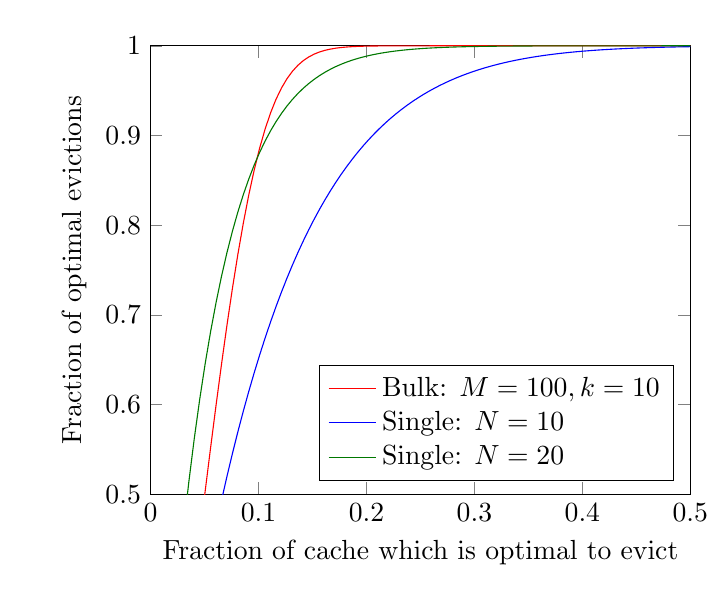
\begin{tikzpicture}
    \definecolor{darkgreen}{RGB}{0,120,0}
    \begin{axis}[
        domain=0:0.5, xmin=0, xmax=0.5,
        range=0.5:1, ymin=0.5, ymax=1,
        samples=100,
        legend pos=south east,
        legend cell align={left},
        xlabel=Fraction of cache which is optimal to evict,
        ylabel=Fraction of optimal evictions,
    ]

    \addplot[color=red]{1 - (1-x)^100 - 90 * x * (1-x)^99 - 3960 * x^2 * (1-x)^98 - 113190 * x^3 * (1-x)^97 - 2352735 * x^4 * (1-x)^96 - 37643760 * x^5 * (1-x)^95 - 476820960 * x^6 * (1-x)^94 - 4802268240 * x^7 * (1-x)^93 - 37217578860 * x^8 * (1-x)^92 - 190223180840 * x^9 * (1-x)^91)};
    % formula expanded with wolframalpha because sums and "choose" function are not available in pgfplot to my knowledge...
    \addlegendentry{Bulk: $M=100, k=10$};
    
    \addplot[color=blue]{1-(1-x)^10};
    \addlegendentry{Single: $N=10$};
    \addplot[color=darkgreen]{1-(1-x)^20};
    \addlegendentry{Single: $N=20$};
    
    \end{axis}
    \end{tikzpicture}
    \caption{Probability of an optimal eviction comparing single- vs bulk-eviction}
    \label{plot:P-opt-bulk-eviction}
\end{figure}

% 

\chapter{Extra results discussion}
About this section: some extra experiments that I think are interesting and may be worth including in the thesis, but maybe not a paper.

\section{CPU overhead}
I do not have very scientific numbers here. General results were: clock-sweep was the lowest ($< 1\mu s$ per eviction), sampling was a bit higher (a few $\mu s$ depending on configuration), PBM-PQ was highest on average but still on the order of 10s of $\mu s$. This is only the time to select the eviction candidates, for PBM it does not include the extra overhead of registering the scans (which will be the same for both PBM forms) or overhead of tracking frequency stats.

There are a few other factors to consider:
\begin{itemize}
    \item Better hit rate means fewer evictions, which could result in less CPU overhead over-all. (or at least reduces the total overhead)
    \item The CPU overhead may scale differently with more parallelism. PBM-PQ likely has more lock contention compared to the others.
\end{itemize}

\section{HDD experiments}
Due to their mechanical design, hard drive performance is highly dependent on the data access pattern. Cache management can indirectly impact the access pattern by influencing \textit{which} accesses go to the disk or not, so the caching policy can impact performance beyond just the hit rate.

Running the same sequential microbenchmarks from Section \ref{sec:eval-seq-micro} on a mechanical HDD, we get similar hit rate and I/O volume results (shown in Figure \ref{fig:hdd_results}) as the SSD, but run-time results that do seem to match these results. Specifically, PBM-sampling consistently achieves less I/O volume but higher run-time than PBM-PQ and Clock-sweep.

\begin{figure*}
    \begin{subfigure}{\textwidth}
        \centering
        \includegraphics[height=0.3\textheight]{figures/hdd_ram_micro/Hit rate vs parallelism - HDD Sequential Scan Microbenchmarks.tikz}
        \caption{HDD Hit Rate}
        \label{fig:hdd_hitrate}
    \end{subfigure}
    \begin{subfigure}{\textwidth}
       \centering
        \includegraphics[height=0.3\textheight]{figures/hdd_ram_micro/IO volume vs parallelism - HDD Sequential Scan Microbenchmarks.tikz}
        \caption{HDD I/O volume}
        \label{fig:hdd_iovol}
    \end{subfigure}
    \begin{subfigure}{\textwidth}
        \centering
        \includegraphics[height=0.3\textheight]{figures/hdd_ram_micro/Time vs parallelism - HDD Sequential Scan Microbenchmarks.tikz}
        \caption{HDD Run-time}
        \label{fig:hdd_time}
    \end{subfigure}
    \caption{HDD Results}
    \label{fig:hdd_results}
\end{figure*}

\begin{figure*}
    \begin{subfigure}{\textwidth}
        \centering
        \includegraphics[height=0.3\textheight]{figures/hdd_ram_micro/Postgres IO rate vs parallelism - HDD Sequential Scan Microbenchmarks.tikz}
        \caption{HDD I/O Throughput}
        \label{fig:hdd_iorate}
    \end{subfigure}  \hspace{0.16\textwidth}
    \begin{subfigure}{\textwidth}
        \centering
        \includegraphics[height=0.3\textheight]{figures/seq_micro/Postgres IO rate vs parallelism - Sequential Scan Microbenchmarks.tikz}
        \caption{SSD I/O Throughput}
        \label{fig:ssd_iorate}
    \end{subfigure}
    \caption{HDD vs SSD I/O Throughput}
\end{figure*}

To understand this, we examine performance metrics for the storage medium itself. Figures \ref{fig:hdd_iorate} and \ref{fig:ssd_iorate} show the I/O throughput of each caching policy using an HDD and SSD respectively.

First, notice that with a mechanical hard drive the I/O throughput decreases as parallelism increases. This can be explained by the access pattern becoming more random; while each scan individually is sequential, multiple scans are not necessarily scanning the same location at the same time and. Compared to the SSD where there is very little performance difference between random and sequential accesses so, I/O throughput continues to increase as parallelism increases and more data is read from the drive, and is not even close to the maximum speed of the drive at low parallelism. 

Comparing the I/O throughput of different caching policies on the HDD, we see that PBM-sampling consistently gets lower throughput than Clock-sweep and PBM-sampling, which are very similar. The most likely explanation here is that the eviction policy is influencing the future access patterns in a way that influences the performance of the drive.

For clock-sweep: for this mostly-sequential workload with no "hot-spots" the algorithm tends to evict blocks in the same order they are accessed, mimicking an LRU strategy. Since all scans access the blocks in the same sequential order, this tends to cause large chunks of the scan to either all be in the cache, or none of it is cached and that whole section can be read sequentially for maximum I/O efficiency. % Compared to the worst-case random policy, where even a sequential scan will frequently alternate between a block that is cached and one that is not. The workload then appears random to the disk, so the IO performance is degraded.

Similarly, PBM-PQ evicts a large number of blocks with similar estimated next access times at once. Blocks from the same region of the table will tend to have similar estimated access times -- especially for this sequential workload -- resulting in large chunks either being entirely cached or entirely not cached.

Here we see that both clock-sweep and PBM-PQ choose eviction candidates in a way that allows accesses \textit{to secondary storage} to be mainly sequential when the queries are accessing data sequentially. In contrast, PBM-sampling evicts single blocks at a time and independently from other evictions. Thus it is fairly likely to have some, but not all, of a range cached requiring a few random reads instead of either having an entire range cached or being able to read the range fully sequentially.

 % With PBM-sampling, it is very possible to have most of a range cached but not some parts, resulting in a few random reads rather than the entire range being cached. Similarly for regions that are mostly not cached, there may be a few blocks in the cache but the cost of reading the extra block from disk would have been low due to the sequential nature of the scan.


For the SSD, IO performance is much more similar among the different strategies. Note that PBM-sampling also gets lower IO throughput, but in this case the IO latency (not shown) is also lower. The reduced throughput is is likely explained by the higher hit rate -- it is simply reading less data and the disk is not fully utilized. PBM-sampling with frequency statistics is a nearly identical strategy but achieves lower hit rate since frequency statistics are not useful for this workload, and has higher IO throughput similar to the other strategies.



\section{Unlimited system memory}
In contrast to experiments with an HDD, we can also run the experiments without limiting the available system memory, so the whole 10 GiB database fits in main memory and is cached by the OS. This has the effect that there is almost no penalty for a PostgreSQL cache miss, so the caching policy does not impact the run-time, but we can still compare the hit rate.

The interesting thing to note compared to the SSD and HDD experiments, is that the hit rate graph flattens out very quickly with every policy and compared to on an SSD where the hit rate increases with parallelism well beyond what is achieved with no cache-miss penalty. Our current hypothesis for why this happens is that the higher penalty for a miss causes scans to automatically synchronize, as discussed in Section \ref{sec:experiment_micro_parallelism}. % When there are two scans on the same relation, the scan that is ahead will be slowed down by cache misses. The scan that is behind may have fewer misses, as all the scan that is ahead has recently read the same data and it is more likely to be in the cache. In this scenario the higher hit rate of the second scan will cause it to scan faster and reduce the gap between the two scans, causing its hit rate to increase even more because there is less time for the data to be evicted between the first and second scan. So the buffer miss penalty causes scans to synchronize increasing the hit rate, while with the whole dataset in-memory the scans are more uniformly distributed so the hit rate is lower.
With the whole data set in-memory, scans do not synchronize in this way so accesses are more uniformly distributed and the hit rate stays low.


% \begin{figure}[ht]
%     \centering
%     \includegraphics[width=0.33\textwidth]{figures/hdd_ram_micro/Time vs parallelism - RAM Sequential Scan Microbenchmarks.tikz}
%     \caption{RAM runtime}
%     \label{fig:ram_time}
% \end{figure}
% \begin{figure}[ht]
%     \centering
%     \includegraphics[width=0.33\textwidth]{figures/hdd_ram_micro/IO volume vs parallelism - RAM Sequential Scan Microbenchmarks.tikz}
%     \caption{RAM IO volume}
%     \label{fig:ram_iovol}
% \end{figure}
\begin{figure}[ht]
    \centering
    \includegraphics[width=0.33\textwidth]{figures/hdd_ram_micro/Hit rate vs parallelism - RAM Sequential Scan Microbenchmarks.tikz}
    \caption{RAM Hit Rate}
    \label{fig:ram_hitrate}
\end{figure}


% GLOSSARIES (Lists of definitions, abbreviations, symbols, etc. provided by the glossaries-extra package)
% -----------------------------
\printglossary
% TODO remove glossary?
\cleardoublepage
\phantomsection		% allows hyperref to link to the correct page

%----------------------------------------------------------------------
\end{document} % end of logical document
